\chapter{Data} \label{cha:chapter-2}

The data I am using for this project is a collection of observations of 5,960 home equity loans which is provided by Baesens, Bart, Roesch, Daniel and Scheule, Harald \cite{baesens2016credit}. Home equity loans are when an applicant borrows agains the value or 'equity' of their home. \textbf{Talk about home equity loans and what they are here.} You can find a full description of each variable in \ref{Table2}.

\begin{figure}[ht]\label{Table2}
	\centering
	\renewcommand{\arraystretch}{1.25}
	\begin{tabular}{l p{6.8cm} p{5cm}}
	\multicolumn{2}{c}{Variables used in the Data Set}\cite{baesens2016credit}\\
	\hline
	Variable & \multicolumn{1}{c}{Definition}\\ 
	\hline
	BAD & 1 = Applicant defaulted on loan or seriously delinquent; 0 = applicant pain load \\
	LOAN & Amount of requested loan \\
	MORTDUE & Amount due on exisiting mortgage \\
	VALUE & Value of property the loan is to go against \\
	REASON & The reason the applicant is applying for the loan. DebtCon = Debt condsolidation; HomeImp = Home Improvement \\
	JOB & Occupational categories \\
	YOJ & Years at present job \\
	DEROG & Number of major derogatory reports \\
	DELINQ & Number of delinquent credit lines \\
	CLAGE & Age of oldest credit line in months \\
	NINQ & Number of recent credit inquiries \\
	CLNO & Number of credit lines \\
	DEBTINC & Debt-to-income ratio \\
	\end{tabular}
\end{figure}

\section{Data Cleaning}

The data provided needed some initial cleaning. 2596 observations were missing atleast one value with some missing several variables. The biggest culprit of this would be DEBTINC with 1,267 missing values. I decided to handle these missing values on a case by case basis applying different methods. First I decided to exclude observations missing more than a third of their variables, 339 fit this criteria. Next before I went forward with any imputing I considered any possible outliers within my numerical data, using the summary table \ref{SUM_BFR_TBL}. You can see for the quantile ranges that there will most likely be some outliers occuring in the majority of the numerical variables. To solve this I removed the 99th percentile for every numerical variable excluding BAD, this ended up removing 589 rows. \\

Moving onto imputing variable, for MORTDUE and VALUE I imputed their values using a simple linear regression of the other. This was going on the assumption that the mortgage due on a house has a strong relationship with the value of property. The assumption is further backed up with the correlation between the two being 0.8748 before imputing, far higher than any of the other correlations in the data.  So for MORTDUE I used (\ref{MORTDUE_IMPUTE}) and for VALUE I used (\ref{VALUE_IMPUTE}). This was applied to any missing value where the other was present and for the remaining I took the mean of each variable from the original data before the imputations.

\begin{equation}\label{MORTDUE_IMPUTE}
\text{MORTDUE} = \beta_{0} + \beta_{1}\text{VALUE}
\end{equation}

\begin{figure}[ht]\label{MORTDUE_IMPUTE_COEFS}
	\centering
	\begin{tabular}{lr}
	\hline
	$\beta_{0}$ & -2145.6497 \\
	$\beta_{1}$ & 0.7177 \\
	\hline
	\end{tabular}
\end{figure}

\begin{equation}\label{VALUE_IMPUTE}
\text{VALUE} = \beta_{0} + \beta_{1}\text{MORTDUE}
\end{equation}

\begin{figure}[ht]\label{VALUE_IMPUTE_COEFS}
	\centering
	\begin{tabular}{lr}
	\hline
	$\beta_{0}$ & 21340.4803 \\
	$\beta_{1}$ & 1.1253 \\
	\hline
	\end{tabular}
\end{figure}

For the remaining numerical variables I chose to take the median of the values as there was no highly correlated variables I could take to impute using linear regression. There is an argument that because DEBTINC is missing 991 (19.7 \%) that some other method from using the median value should be used but the only reasonable solution with the data available would be to drop the variable all together or drop the missing rows, both would result in a large loss of data. As this will most likely have a significant impact on the importance of the variable I planned to look into the performance of a few datasets with different solutions for this variable. \\

Last was the two categorical variables REASON ( DebtCon, HomeImp ) and JOB ( Other, Office, Sales, Mgr, ProfExe, Self ). REASON's categories were specified in the data dictionary but JOB's categories were not, for simplicity I am going to assume that the missing values are of the categories just specified. Their missing values were 138 and 127 respectively and I decided to impute these values using a weighted random sample with the weights being the counts of the respective category. Below is two table summarizing the imputes, I applied a seed to reproduce the sampling to remian consistent. 

\begin{figure}[ht]\label{REASON_IMPUTES}
	\centering
	\renewcommand{\arraystretch}{1.25}
	\begin{tabular}{lrrrr}
	\multicolumn{5}{c}{REASON}\\
	\hline
	Category & \multicolumn{1}{c}{Original} & \multicolumn{1}{c}{Weight For Sampling} & \multicolumn{1}{c}{New} & \multicolumn{1}{c}{Count Imputed} \\ 
	\hline
	DebtCon & 3448 & 0.7005 & 3528 & 80\\
	HomeImp & 1474 & 0.2995 & 1504  & 30\\
	\end{tabular}
\end{figure}

\begin{figure}[ht]\label{JOB_IMPUTES}
	\centering
	\renewcommand{\arraystretch}{1.25}
	\begin{tabular}{lrrrr}
	\multicolumn{5}{c}{JOB}\\
	\hline
	Category & \multicolumn{1}{c}{Original} & \multicolumn{1}{c}{Weight For Sampling} & \multicolumn{1}{c}{New} & \multicolumn{1}{c}{Count Imputed} \\ 
	\hline
	Other & 2056 & 0.4175 & 2100 & 44 \\
	ProfExe & 1123 & 0.2281 & 1150 & 27 \\
	Office & 862 & 0.1751 & 877 & 15 \\
	Mgr & 646 & 0.1312 & 657  & 11 \\
	Self & 144 & 0.0292 & 151  & 7 \\
	Sales & 93 & 0.0189 & 97 & 4 \\
	\end{tabular}
\end{figure}

With these two completed I had no more missing values an no other noticeable issues which needed to be corrected before I could further look into the variables. A summary of actions taken on missing values can be found in table (\ref{data_clean})

\begin{figure}[ht]\label{data_clean}
	\centering
	\renewcommand{\arraystretch}{1.25}
	\begin{tabular}{l p{3cm} p{9cm}}
	\multicolumn{3}{c}{Missing Variables Breakdown}\\
	\hline
	Variable & \multicolumn{1}{c}{No. Missing} & \multicolumn{1}{c}{Solution}\\ 
	\hline
	BAD & 0 & N/A\\
	LOAN & 0 & N/A \\
	MORTDUE & 316 & Imputed from a linear regression (\ref{MORTDUE_IMPUTE}). Mean taken when VALUE was unavailable \\
	VALUE & 59 & Imputed from a linear regression (\ref{VALUE_IMPUTE}). Mean taken when MORTDUE was unavailable \\
	REASON & 110 & Random weighted sample taken \\
	JOB & 108 & Random weighted sample taken \\
	YOJ & 311 & Median taken\\
	DEROG & 362 & Median taken \\
	DELINQ & 246 & Median taken\\
	CLAGE & 67 & Median taken \\
	NINQ & 178 & Median taken\\
	CLNO & 0 & N/A \\
	DEBTINC & 991 & Median taken\\
	\end{tabular}
\end{figure}

\begin{landscape}
\begin{figure}[ht]
	\centering
	\renewcommand{\arraystretch}{2}
	\begin{tabular}{lrrrrrrrrrrr}
	\toprule
	{} &     BAD &      LOAN &    MORTDUE &      VALUE &      YOJ &    DEROG &   DELINQ &    CLAGE &     NINQ &     CLNO &  DEBTINC \\
	\midrule
	count &  5621.0 &   5621.00 &    5278.00 &    5537.00 &  5294.00 &  5206.00 &  5356.00 &  5549.00 &  5422.00 &  5621.00 &  4447.00 \\
	mean  &     0.2 &  18846.02 &   73977.01 &  103025.40 &     9.00 &     0.24 &     0.45 &   179.77 &     1.19 &    21.45 &    34.07 \\
	std   &     0.4 &  11301.47 &   44813.54 &   58002.35 &     7.61 &     0.80 &     1.13 &    85.70 &     1.73 &    10.13 &     8.47 \\
	min   &     0.0 &   1100.00 &    2063.00 &    8000.00 &     0.00 &     0.00 &     0.00 &     0.00 &     0.00 &     0.00 &     0.52 \\
	25\%   &     0.0 &  11300.00 &   46385.00 &   66922.00 &     3.00 &     0.00 &     0.00 &   115.57 &     0.00 &    15.00 &    29.43 \\
	50\%   &     0.0 &  16500.00 &   65000.00 &   90008.00 &     7.00 &     0.00 &     0.00 &   173.63 &     1.00 &    20.00 &    35.02 \\
	75\%   &     0.0 &  23500.00 &   91989.25 &  120724.00 &    13.00 &     0.00 &     0.00 &   230.72 &     2.00 &    26.00 &    39.14 \\
	max   &     1.0 &  89900.00 &  399550.00 &  855909.00 &    41.00 &    10.00 &    15.00 &  1168.23 &    17.00 &    71.00 &   203.31 \\
	\bottomrule
	\end{tabular}
	\caption{Summary Before Outliers Removed \label{SUM_BFR_TBL}}
\end{figure}
\end{landscape}

\begin{landscape}
\begin{figure}[ht]
	\centering
	\renewcommand{\arraystretch}{2}
	\begin{tabular}{lrrrrrrrrrrr}
	\toprule
	{} &      BAD &      LOAN &    MORTDUE &      VALUE &      YOJ &    DEROG &   DELINQ &    CLAGE &     NINQ &     CLNO &  DEBTINC \\
	\midrule
	mean  &     0.17 &  17944.69 &   68427.20 &   98341.35 &     8.60 &     0.15 &     0.32 &   174.81 &     1.04 &    20.65 &    33.88 \\
	std   &     0.38 &   9547.25 &   36656.24 &   45860.89 &     6.95 &     0.49 &     0.77 &    76.09 &     1.35 &     9.08 &     6.11 \\
	min   &     0.00 &   1100.00 &    2063.00 &    8000.00 &     0.00 &     0.00 &     0.00 &     0.51 &     0.00 &     0.00 &     0.52 \\
	25\%   &     0.00 &  11100.00 &   44317.25 &   66343.75 &     3.00 &     0.00 &     0.00 &   114.59 &     0.00 &    14.00 &    30.94 \\
	50\%   &     0.00 &  16200.00 &   62562.50 &   89033.00 &     7.00 &     0.00 &     0.00 &   170.72 &     1.00 &    20.00 &    34.88 \\
	75\%   &     0.00 &  22725.00 &   87368.50 &  117696.75 &    12.00 &     0.00 &     0.00 &   225.11 &     2.00 &    26.00 &    37.97 \\
	max   &     1.00 &  62700.00 &  207687.00 &  271738.00 &    29.00 &     3.00 &     4.00 &   398.40 &     7.00 &    48.00 &    48.28 \\
	\bottomrule
	\end{tabular}
	\caption{Summary After Outliers Removed \label{SUM_AFT_TBL}}
\end{figure}
\end{landscape}

\begin{landscape}
\begin{figure}[ht]
	\centering
	\renewcommand{\arraystretch}{2}
	\begin{tabular}{lrrrrrrrrrrr}
		\toprule
		{} &    BAD &   LOAN &  MORTDUE &  VALUE &    YOJ &  DEROG &  DELINQ &  CLAGE &   NINQ &   CLNO &  DEBTINC \\
		\midrule
		BAD     &  1.000 & -0.073 &   -0.031 & -0.033 & -0.065 &  0.297 &   0.354 & -0.170 &  0.173 & -0.010 &    0.155 \\
		LOAN    & -0.073 &  1.000 &    0.228 &  0.332 &  0.093 & -0.032 &  -0.037 &  0.097 &  0.043 &  0.069 &    0.062 \\
		MORTDUE & -0.031 &  0.228 &    1.000 &  0.895 & -0.064 & -0.047 &   0.002 &  0.128 &  0.027 &  0.331 &    0.146 \\
		VALUE   & -0.033 &  0.332 &    0.895 &  1.000 &  0.003 & -0.043 &  -0.004 &  0.173 & -0.006 &  0.261 &    0.099 \\
		YOJ     & -0.065 &  0.093 &   -0.064 &  0.003 &  1.000 & -0.060 &   0.047 &  0.190 & -0.066 &  0.023 &   -0.066 \\
		DEROG   &  0.297 & -0.032 &   -0.047 & -0.043 & -0.060 &  1.000 &   0.176 & -0.073 &  0.156 &  0.054 &    0.028 \\
		DELINQ  &  0.354 & -0.037 &    0.002 & -0.004 &  0.047 &  0.176 &   1.000 &  0.027 &  0.055 &  0.157 &    0.042 \\
		CLAGE   & -0.170 &  0.097 &    0.128 &  0.173 &  0.190 & -0.073 &   0.027 &  1.000 & -0.112 &  0.237 &   -0.049 \\
		NINQ    &  0.173 &  0.043 &    0.027 & -0.006 & -0.066 &  0.156 &   0.055 & -0.112 &  1.000 &  0.082 &    0.120 \\
		CLNO    & -0.010 &  0.069 &    0.331 &  0.261 &  0.023 &  0.054 &   0.157 &  0.237 &  0.082 &  1.000 &    0.143 \\
		DEBTINC &  0.155 &  0.062 &    0.146 &  0.099 & -0.066 &  0.028 &   0.042 & -0.049 &  0.120 &  0.143 &    1.000 \\
		\bottomrule
	\end{tabular}
	\caption{Correlation Table \label{CORR_TBL}}
\end{figure}
\end{landscape}

\section{Variables}

With the data cleaned I then was able to look more into the properties of the variables and their relationship with the default outcome. First looking at the summary data found in Table
 \ref{SUM_TBL}

\begin{figure}[!ht]
	\centering
	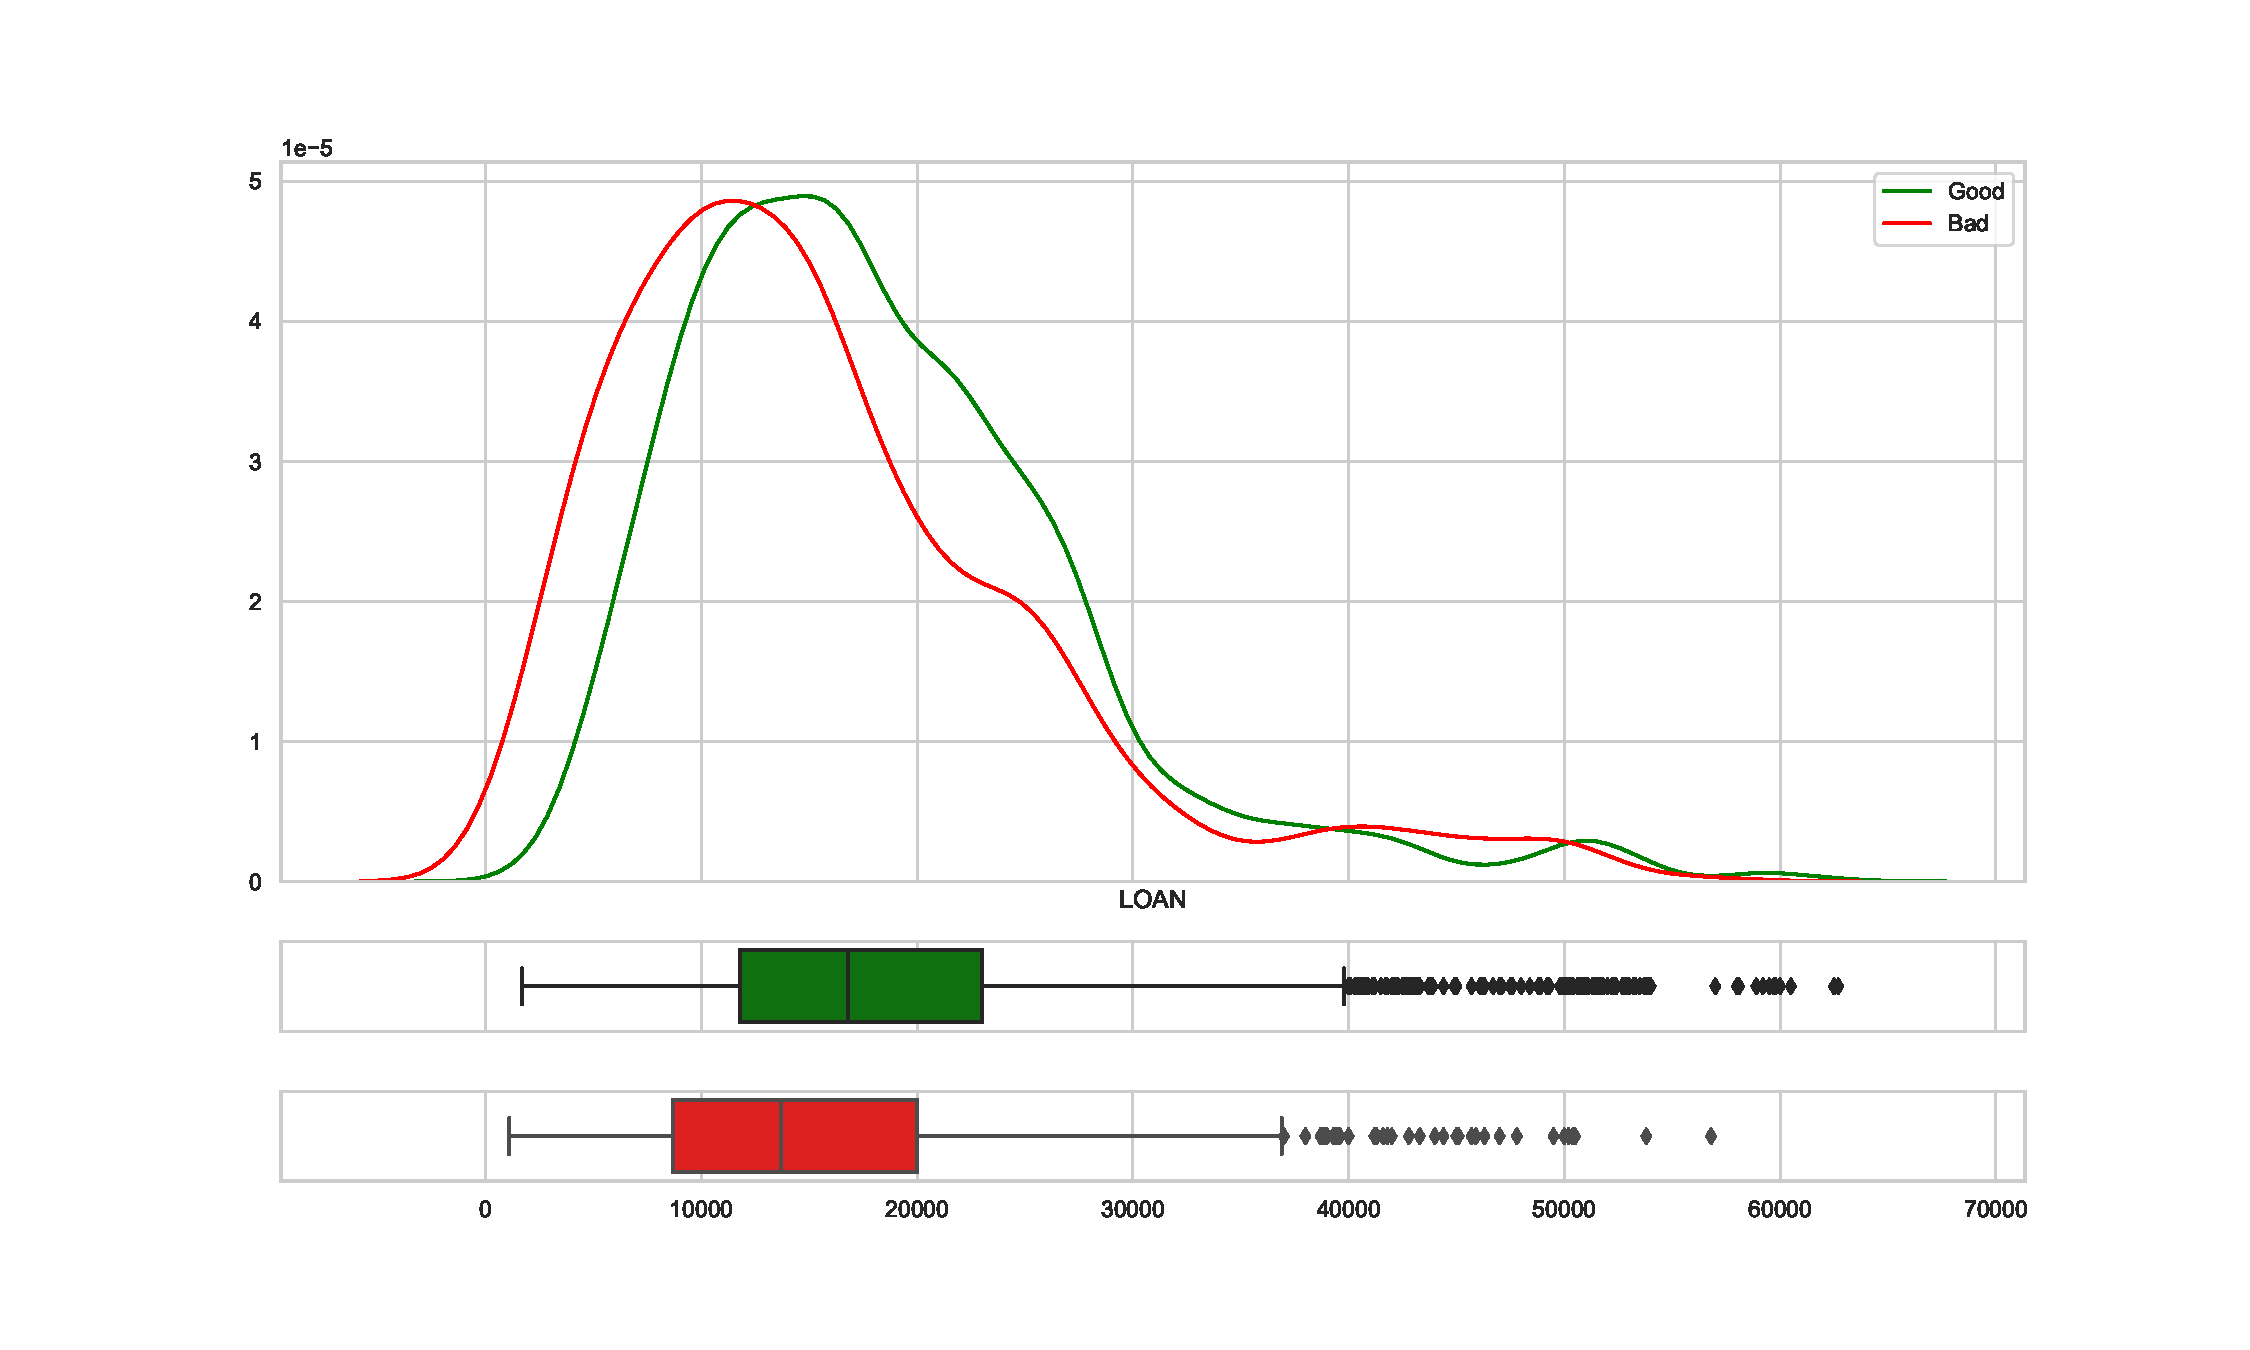
\includegraphics[scale=0.40]{figs/loan_dist.pdf}
	\caption{Distribution of LOAN by BAD. \label{loan_dist}}
\end{figure}

\begin{figure}[!ht]
	\centering
	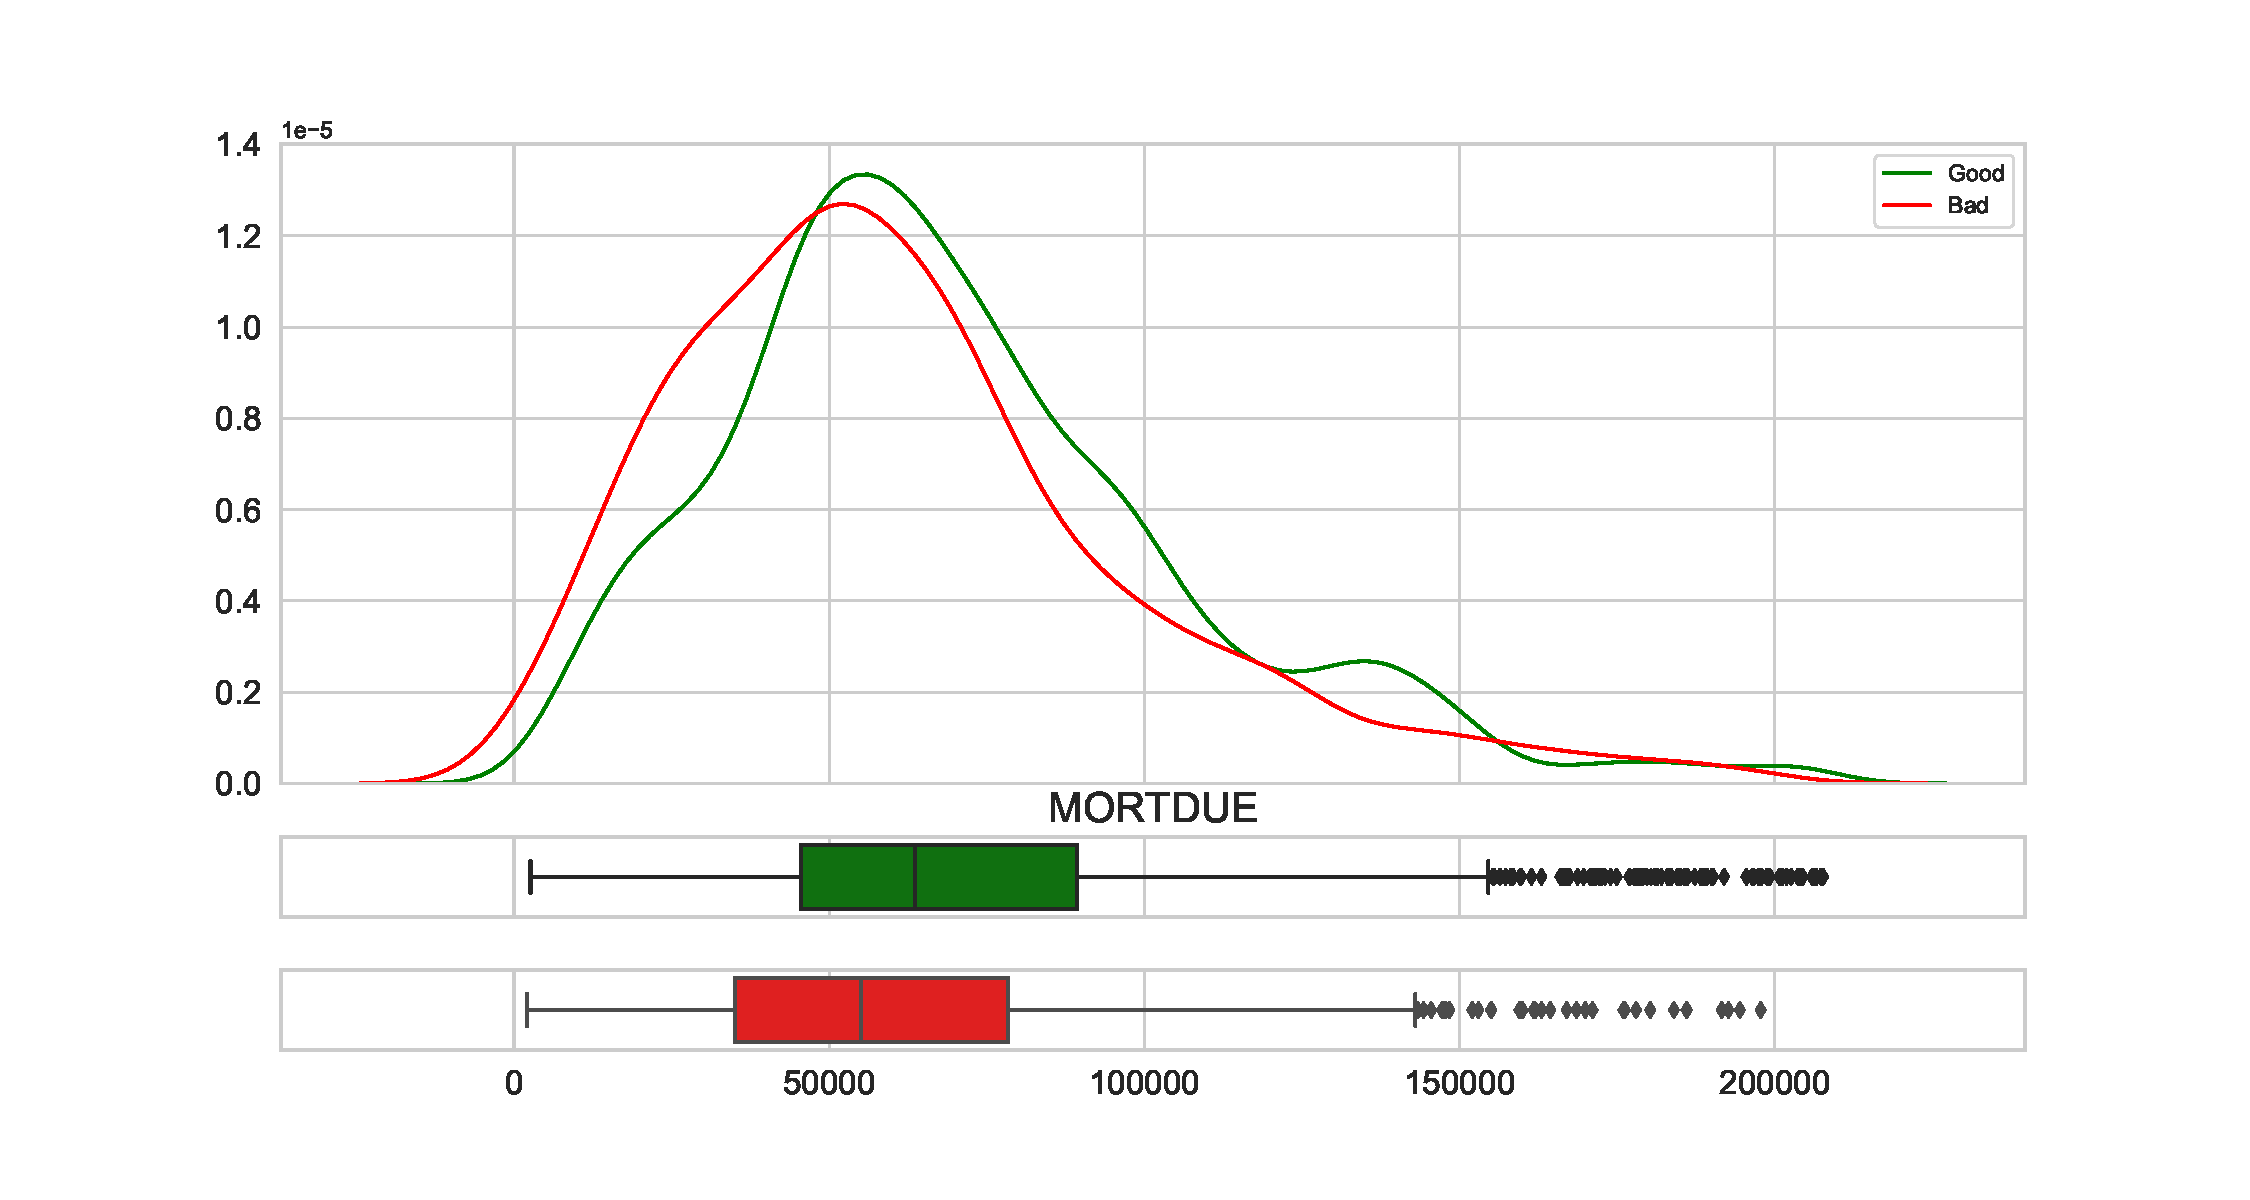
\includegraphics[scale=0.40]{figs/mortdue_dist.pdf}
	\caption{Distribution of MORTDUE by BAD. \label{mortdue_dist}}
\end{figure}

\begin{figure}[!ht]
	\centering
	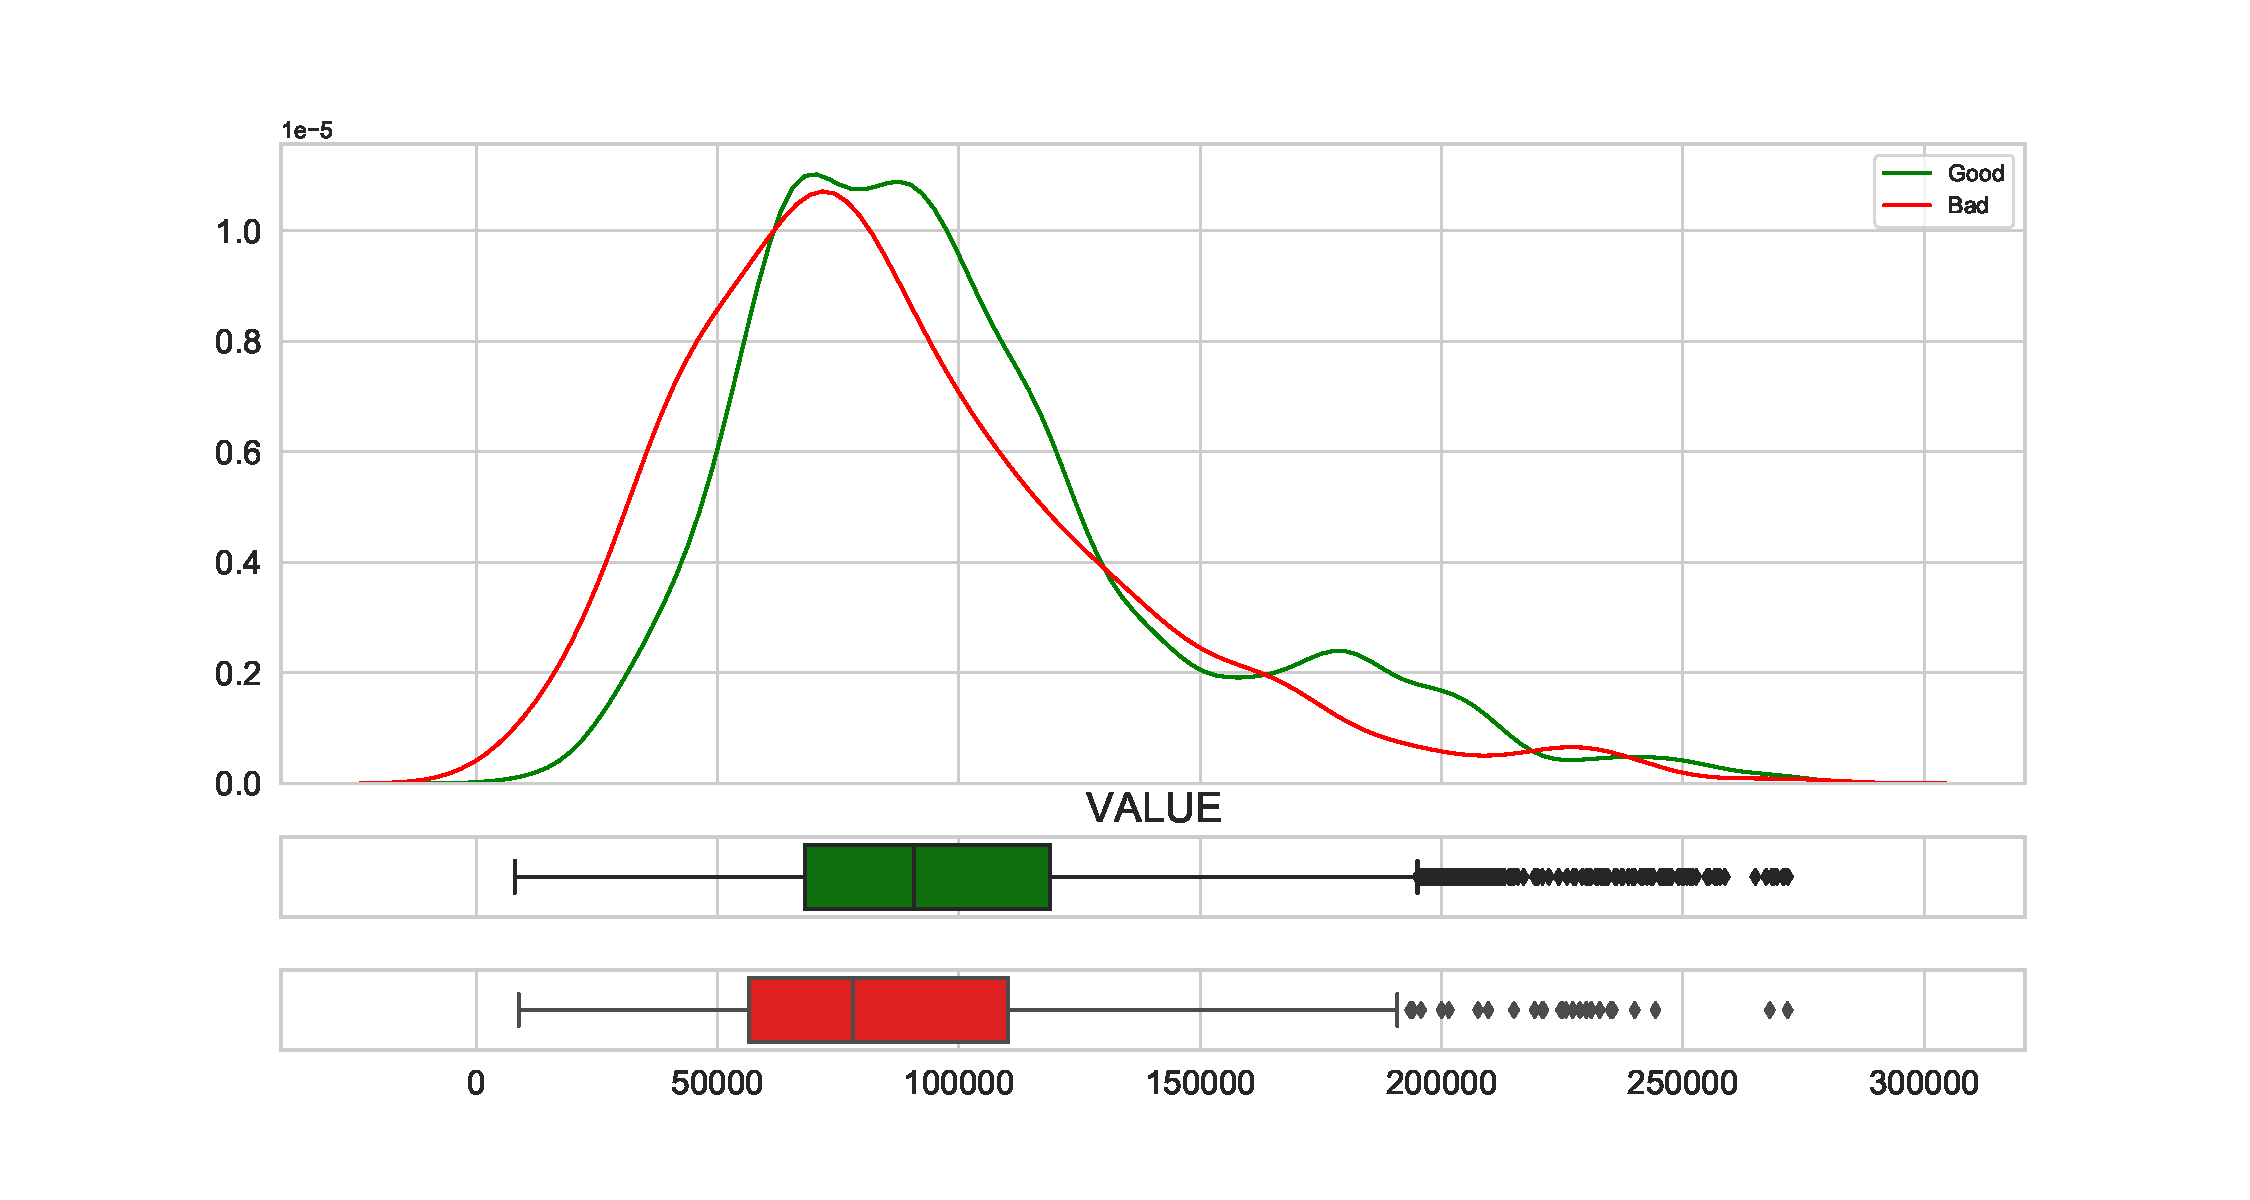
\includegraphics[scale=0.40]{figs/value_dist.pdf}
	\caption{Distribution of VALUE by BAD. \label{value_dist}}
\end{figure}

\begin{figure}[!ht]
	\centering
	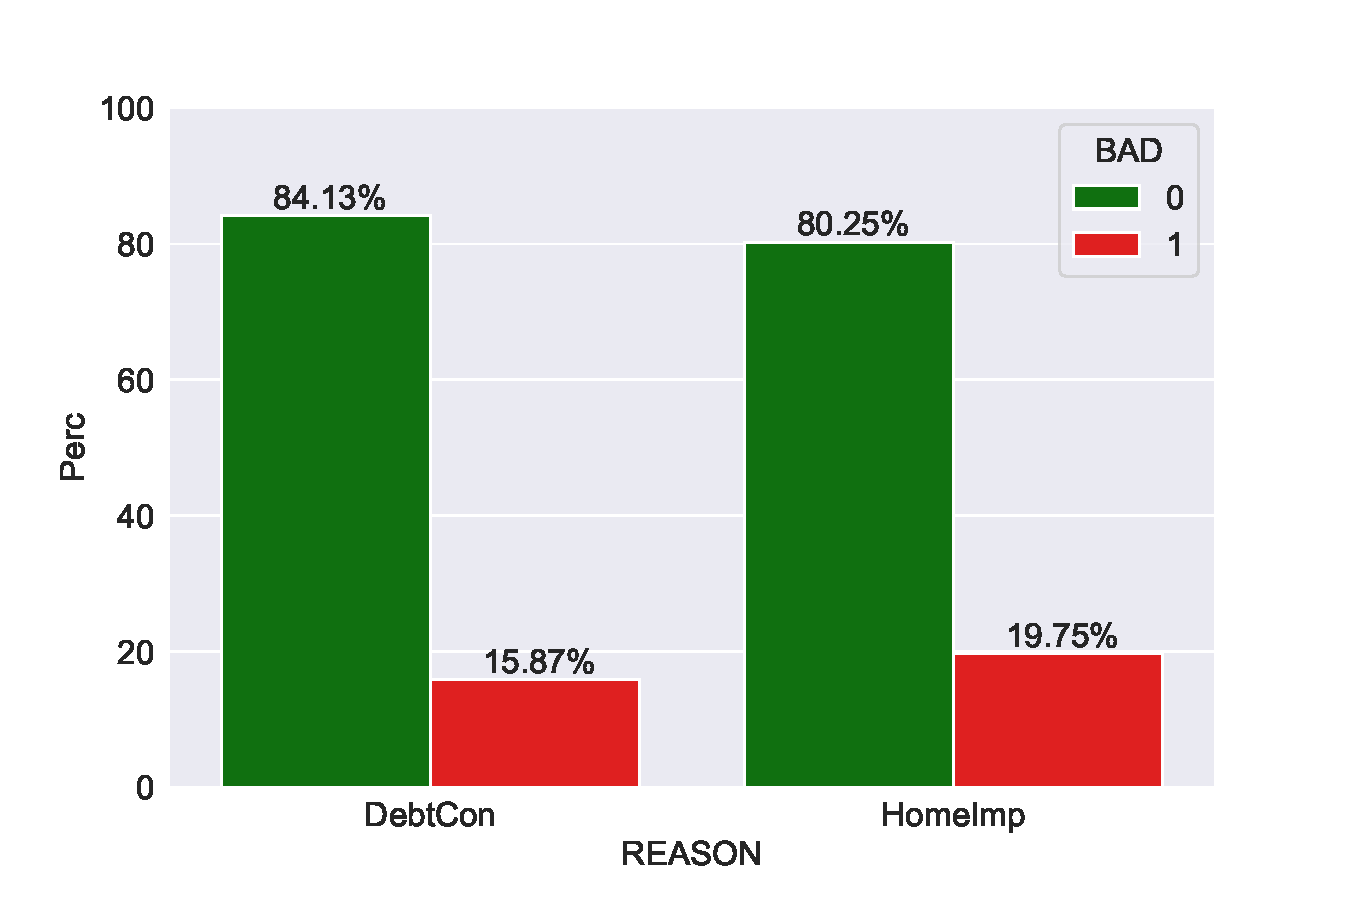
\includegraphics[scale=0.40]{figs/reason_cat.pdf}
	\caption{Category plot of REASON by BAD. \label{reason_cat}}
\end{figure}

\begin{figure}[!ht]
	\centering
	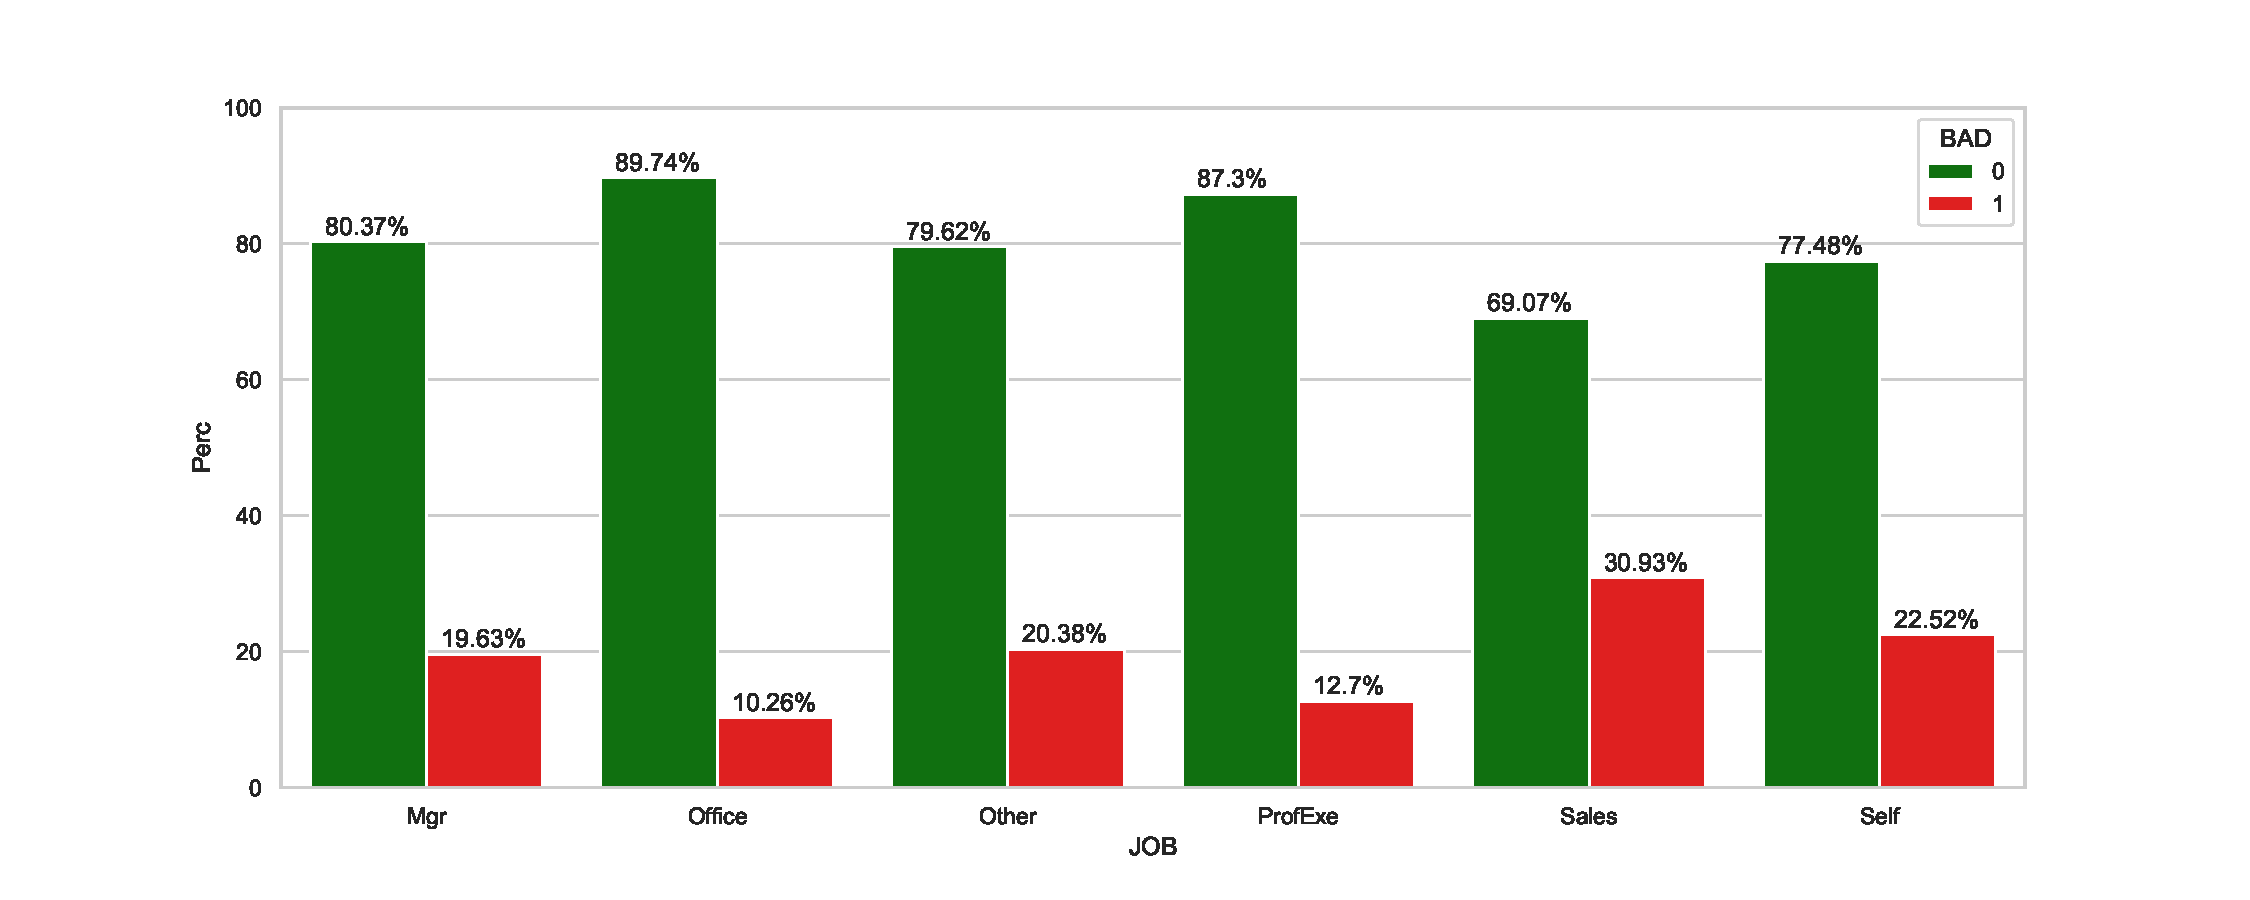
\includegraphics[scale=0.40]{figs/job_cat.pdf}
	\caption{Category plot of JOB by BAD. \label{job_cat}}
\end{figure}

\begin{figure}[!ht]
	\centering
	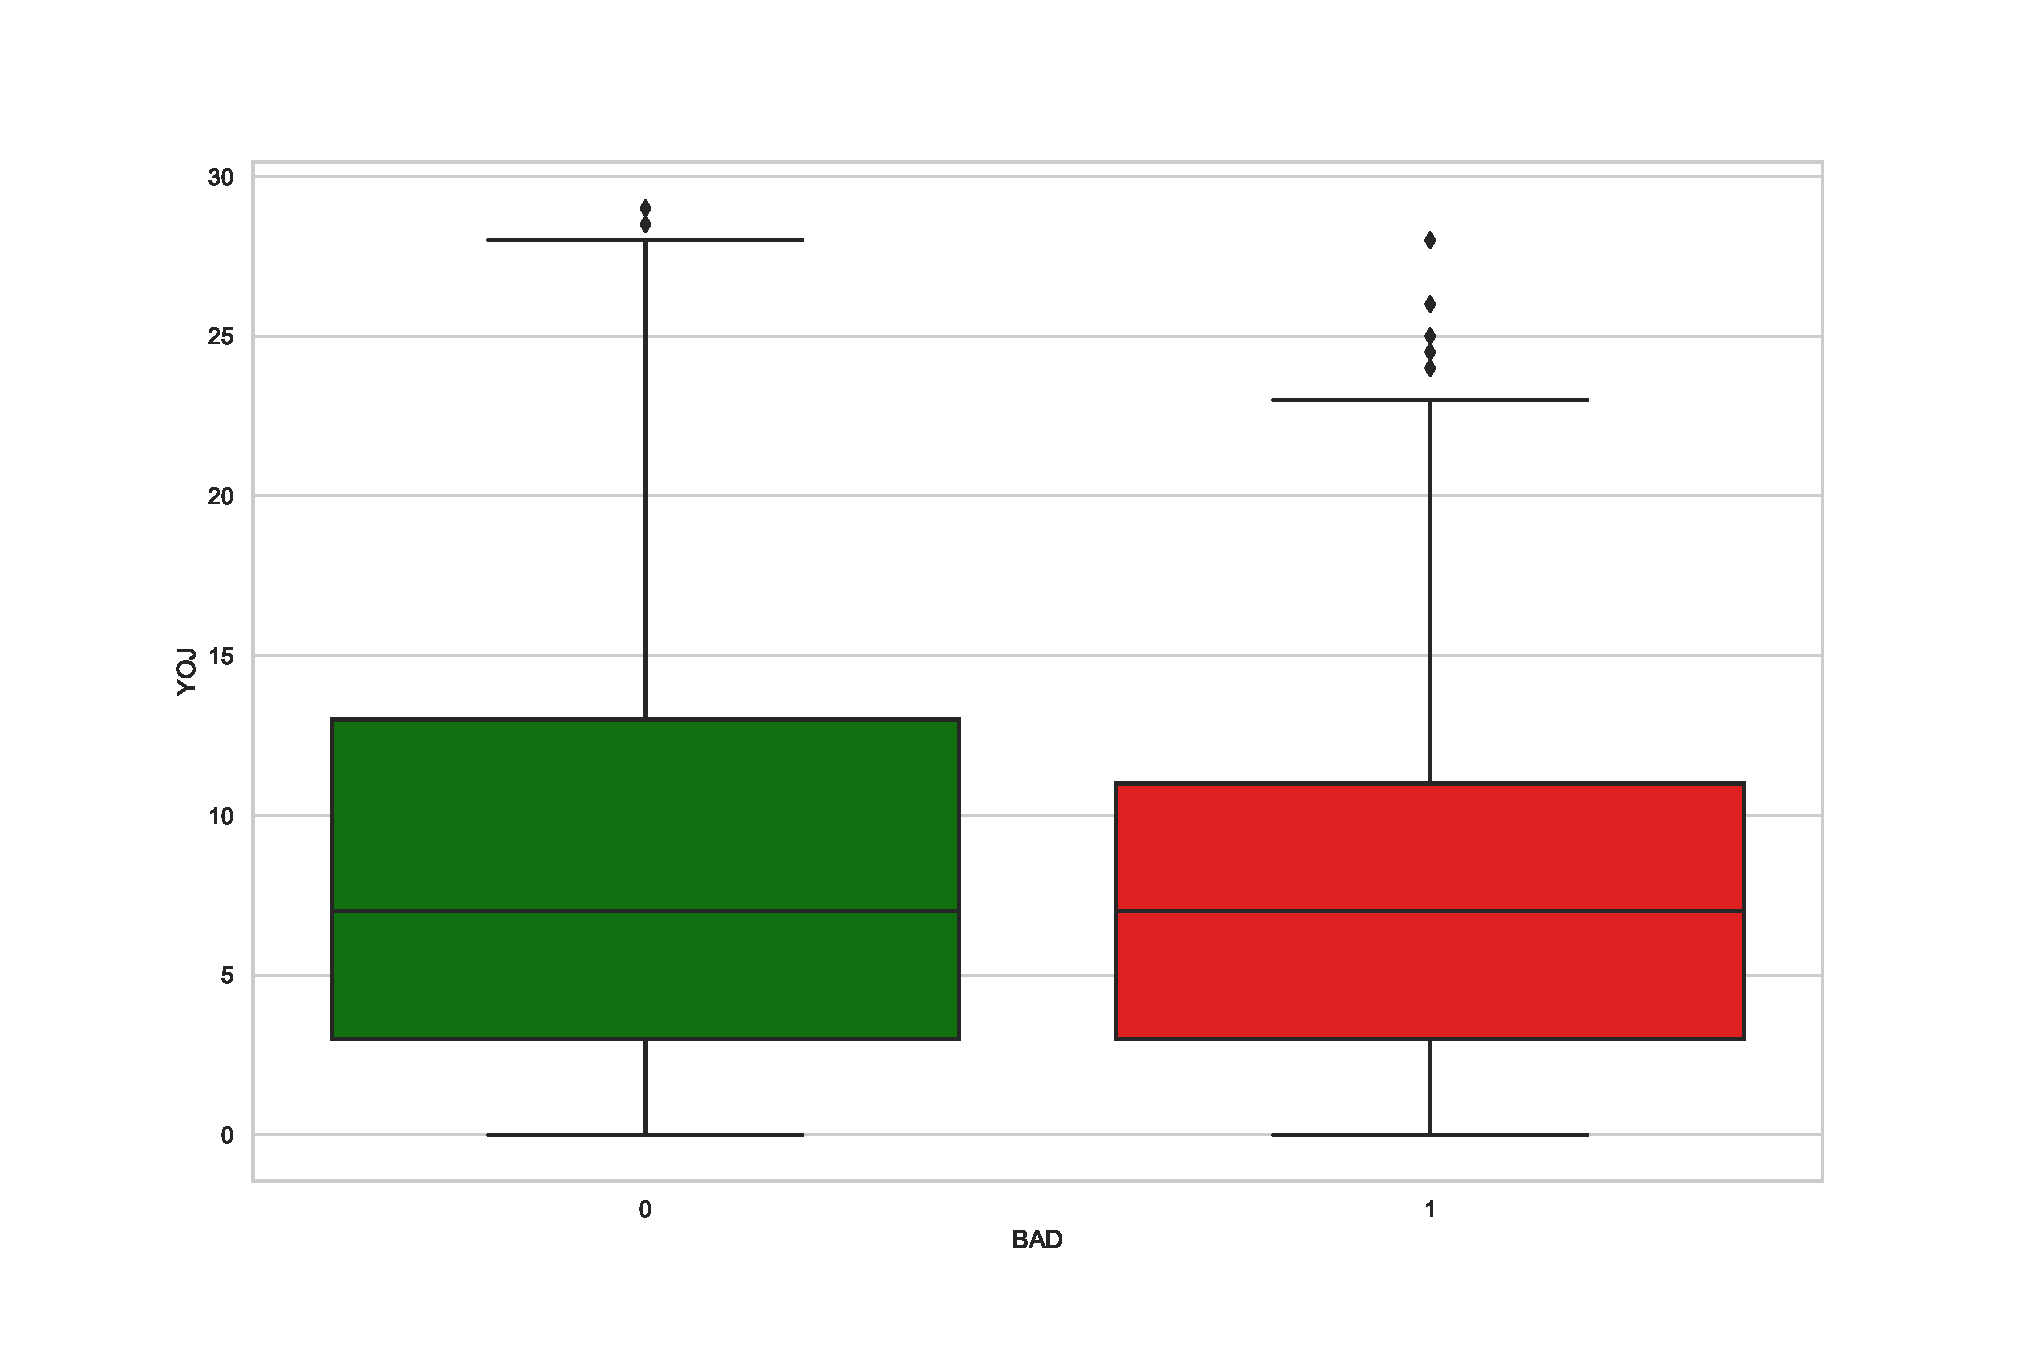
\includegraphics[scale=0.40]{figs/yoj_box.pdf}
	\caption{Boxplot of YOJ by BAD. \label{yoj_box}}
\end{figure}

\begin{figure}[!ht]
	\centering
	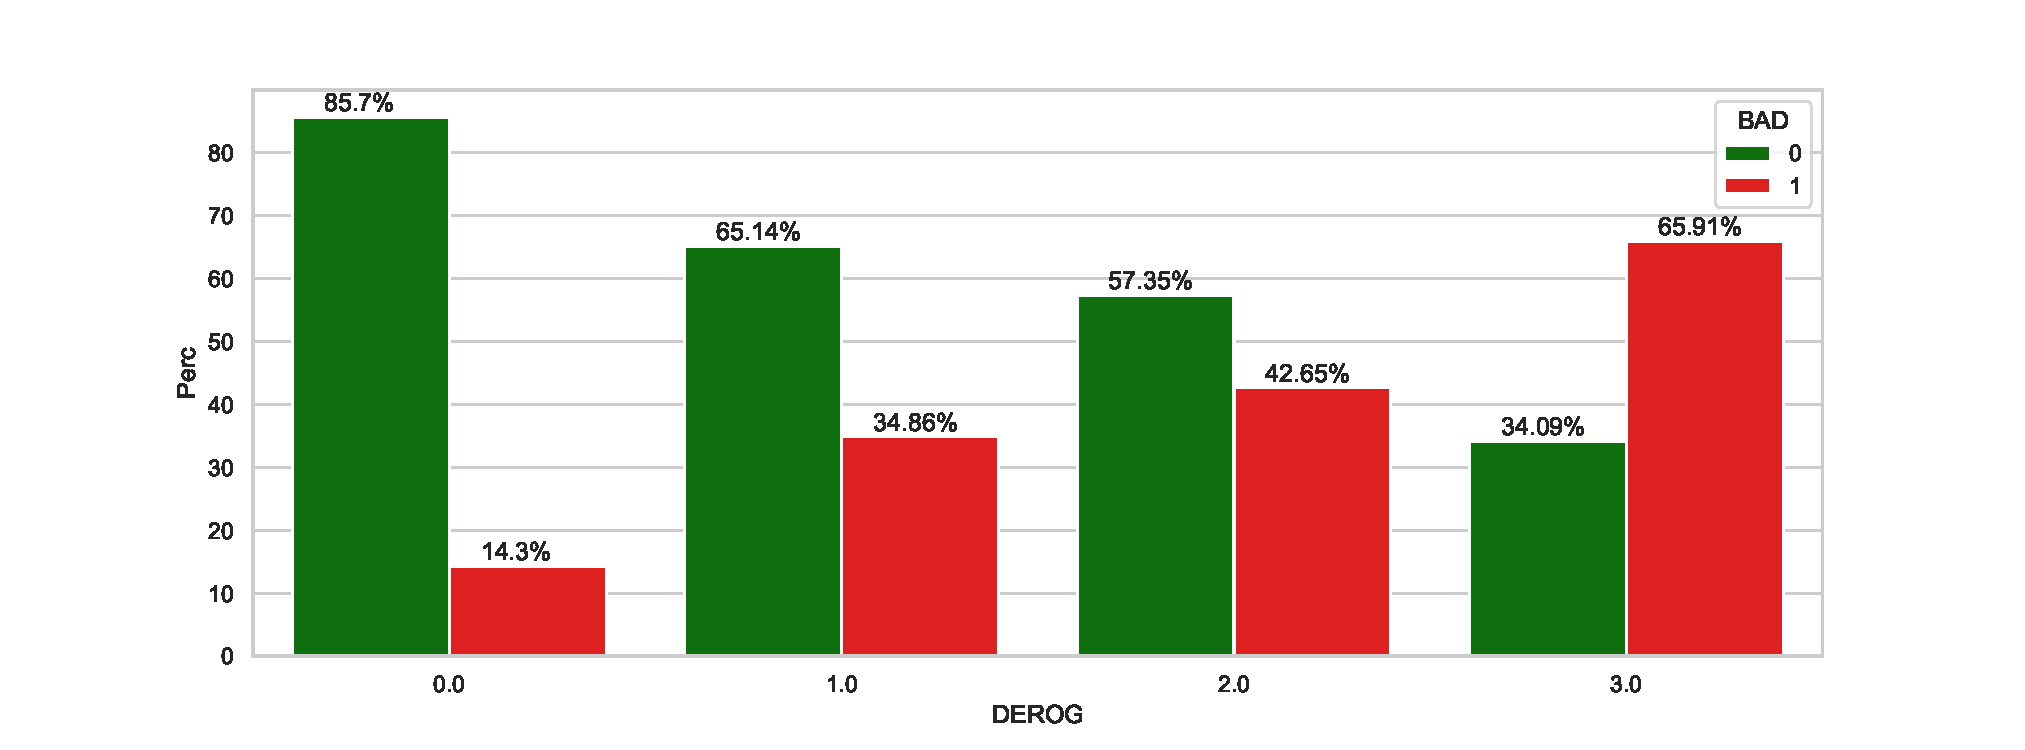
\includegraphics[scale=0.40]{figs/derog_cat.pdf}
	\caption{Category plot of DEROG by BAD. \label{derog_cat}}
\end{figure}

\begin{figure}[!ht]
	\centering
	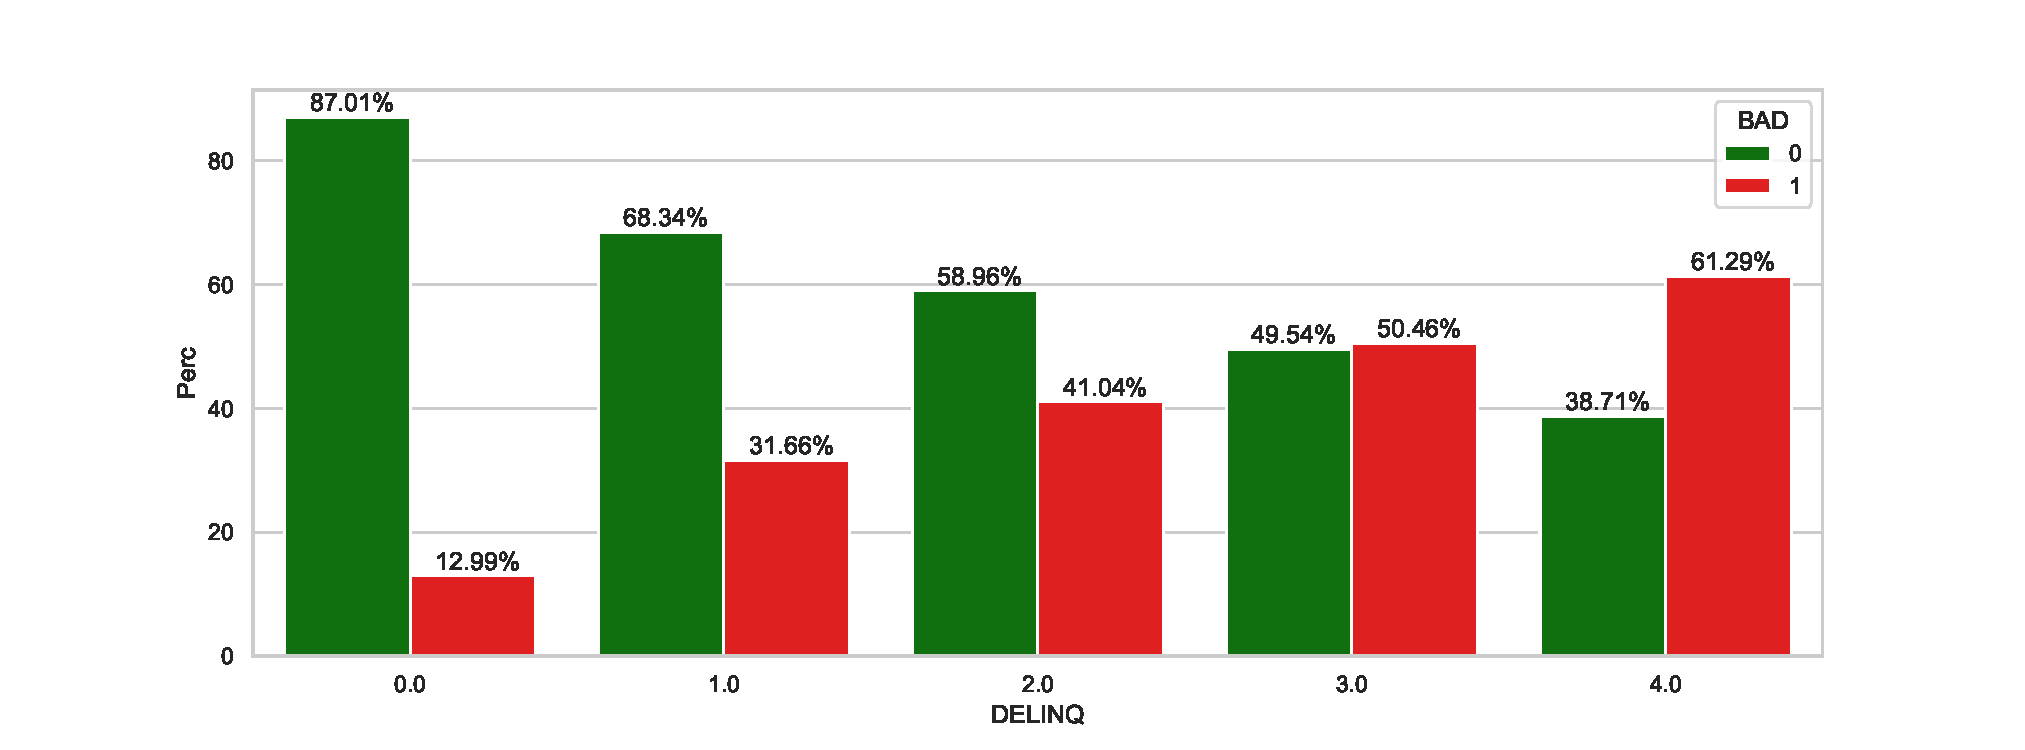
\includegraphics[scale=0.40]{figs/delinq_cat.pdf}
	\caption{Category plot of DELINQ by BAD. \label{delinq_cat}}
\end{figure}

\begin{figure}[!ht]
	\centering
	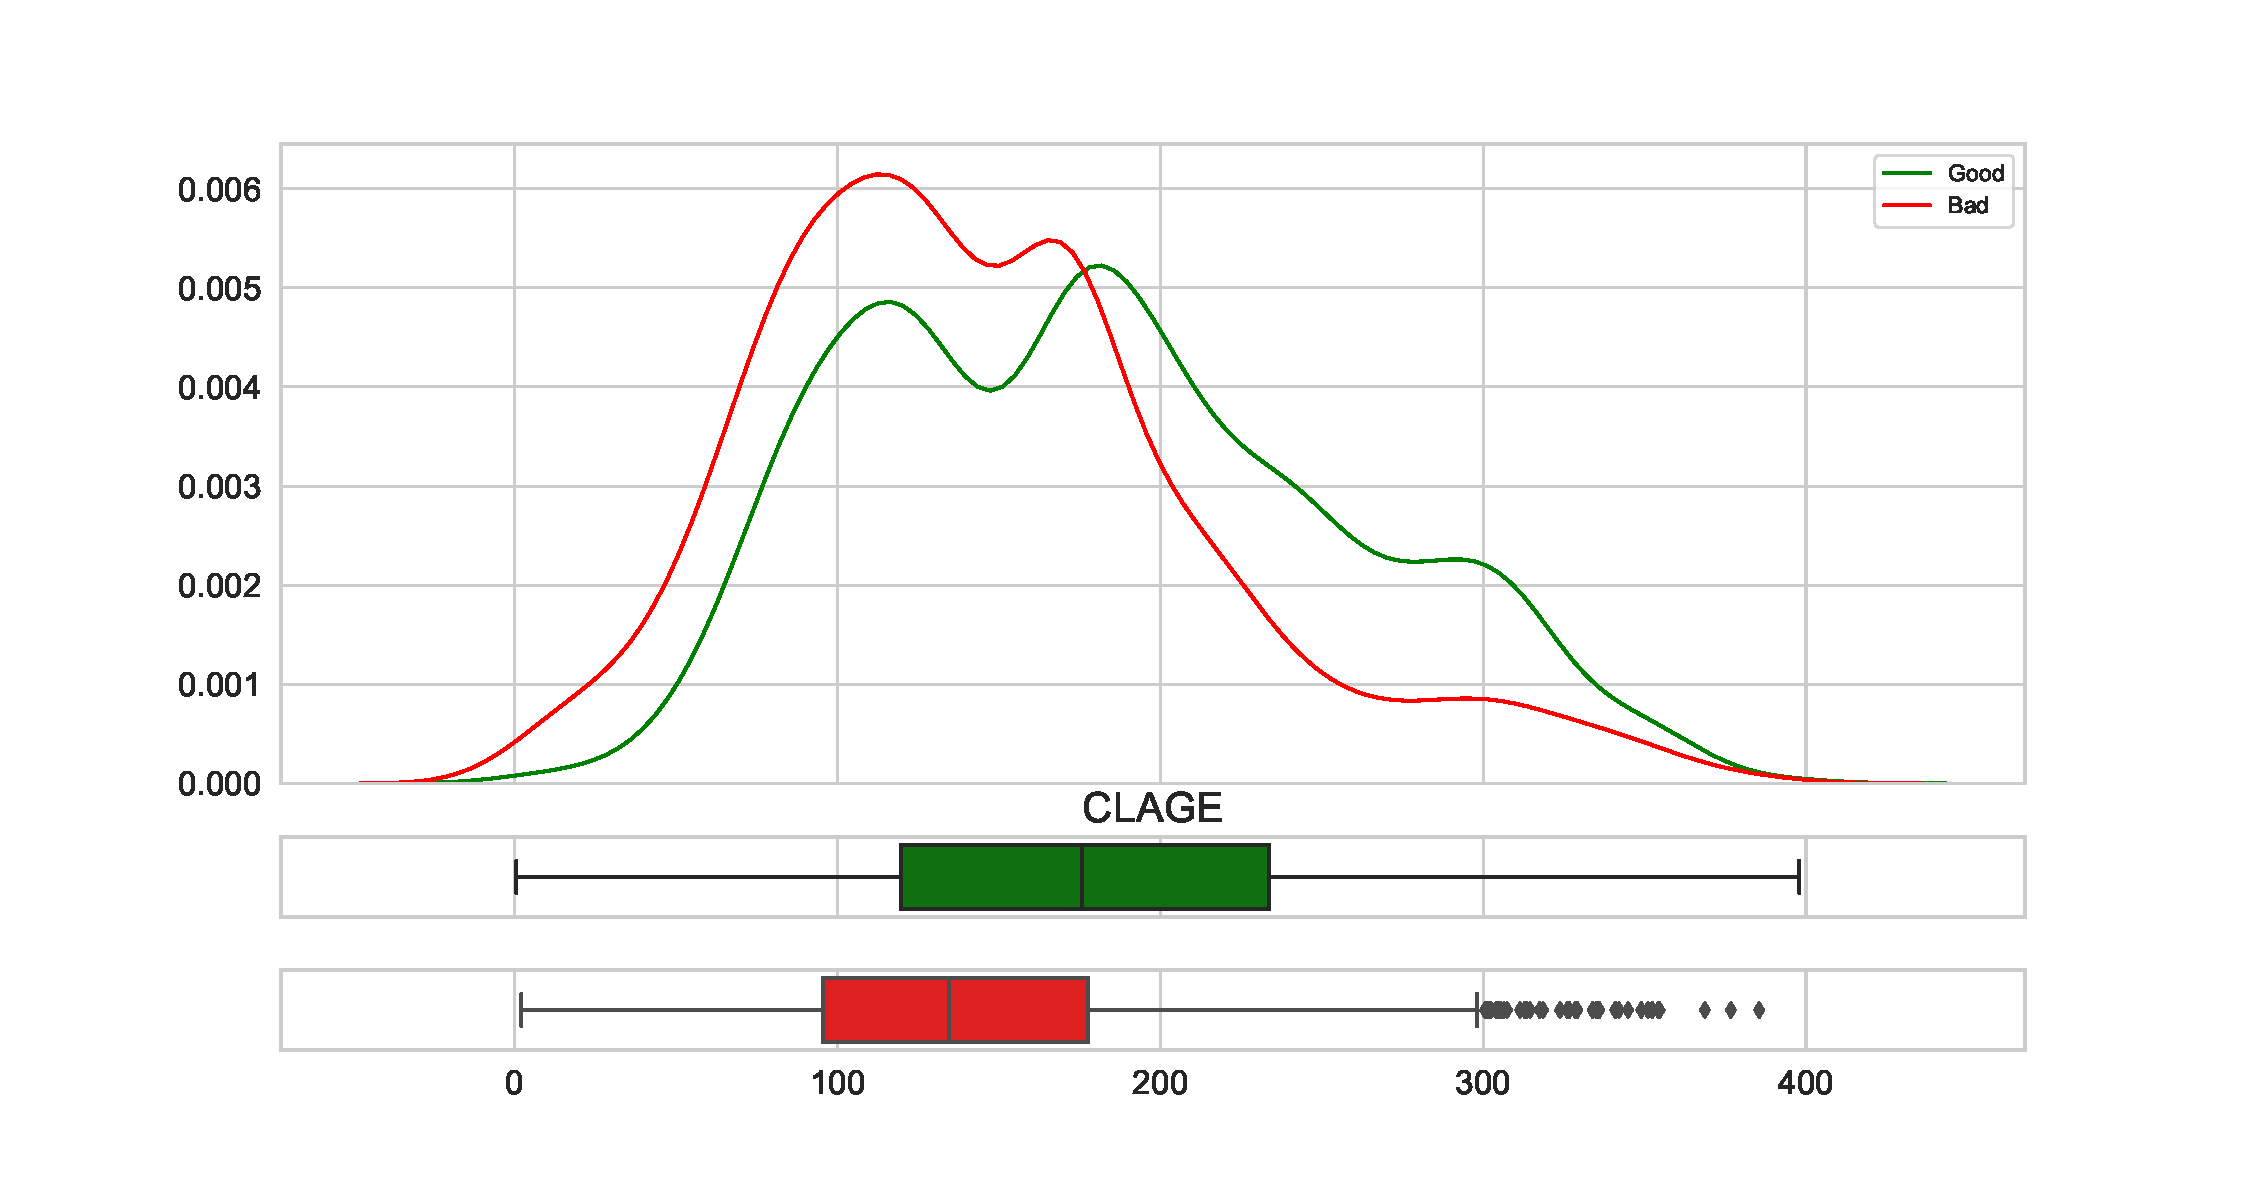
\includegraphics[scale=0.40]{figs/clage_dist.pdf}
	\caption{Distribution of CLAGE by BAD. \label{clage_dist}}
\end{figure}

\begin{figure}[!ht]
	\centering
	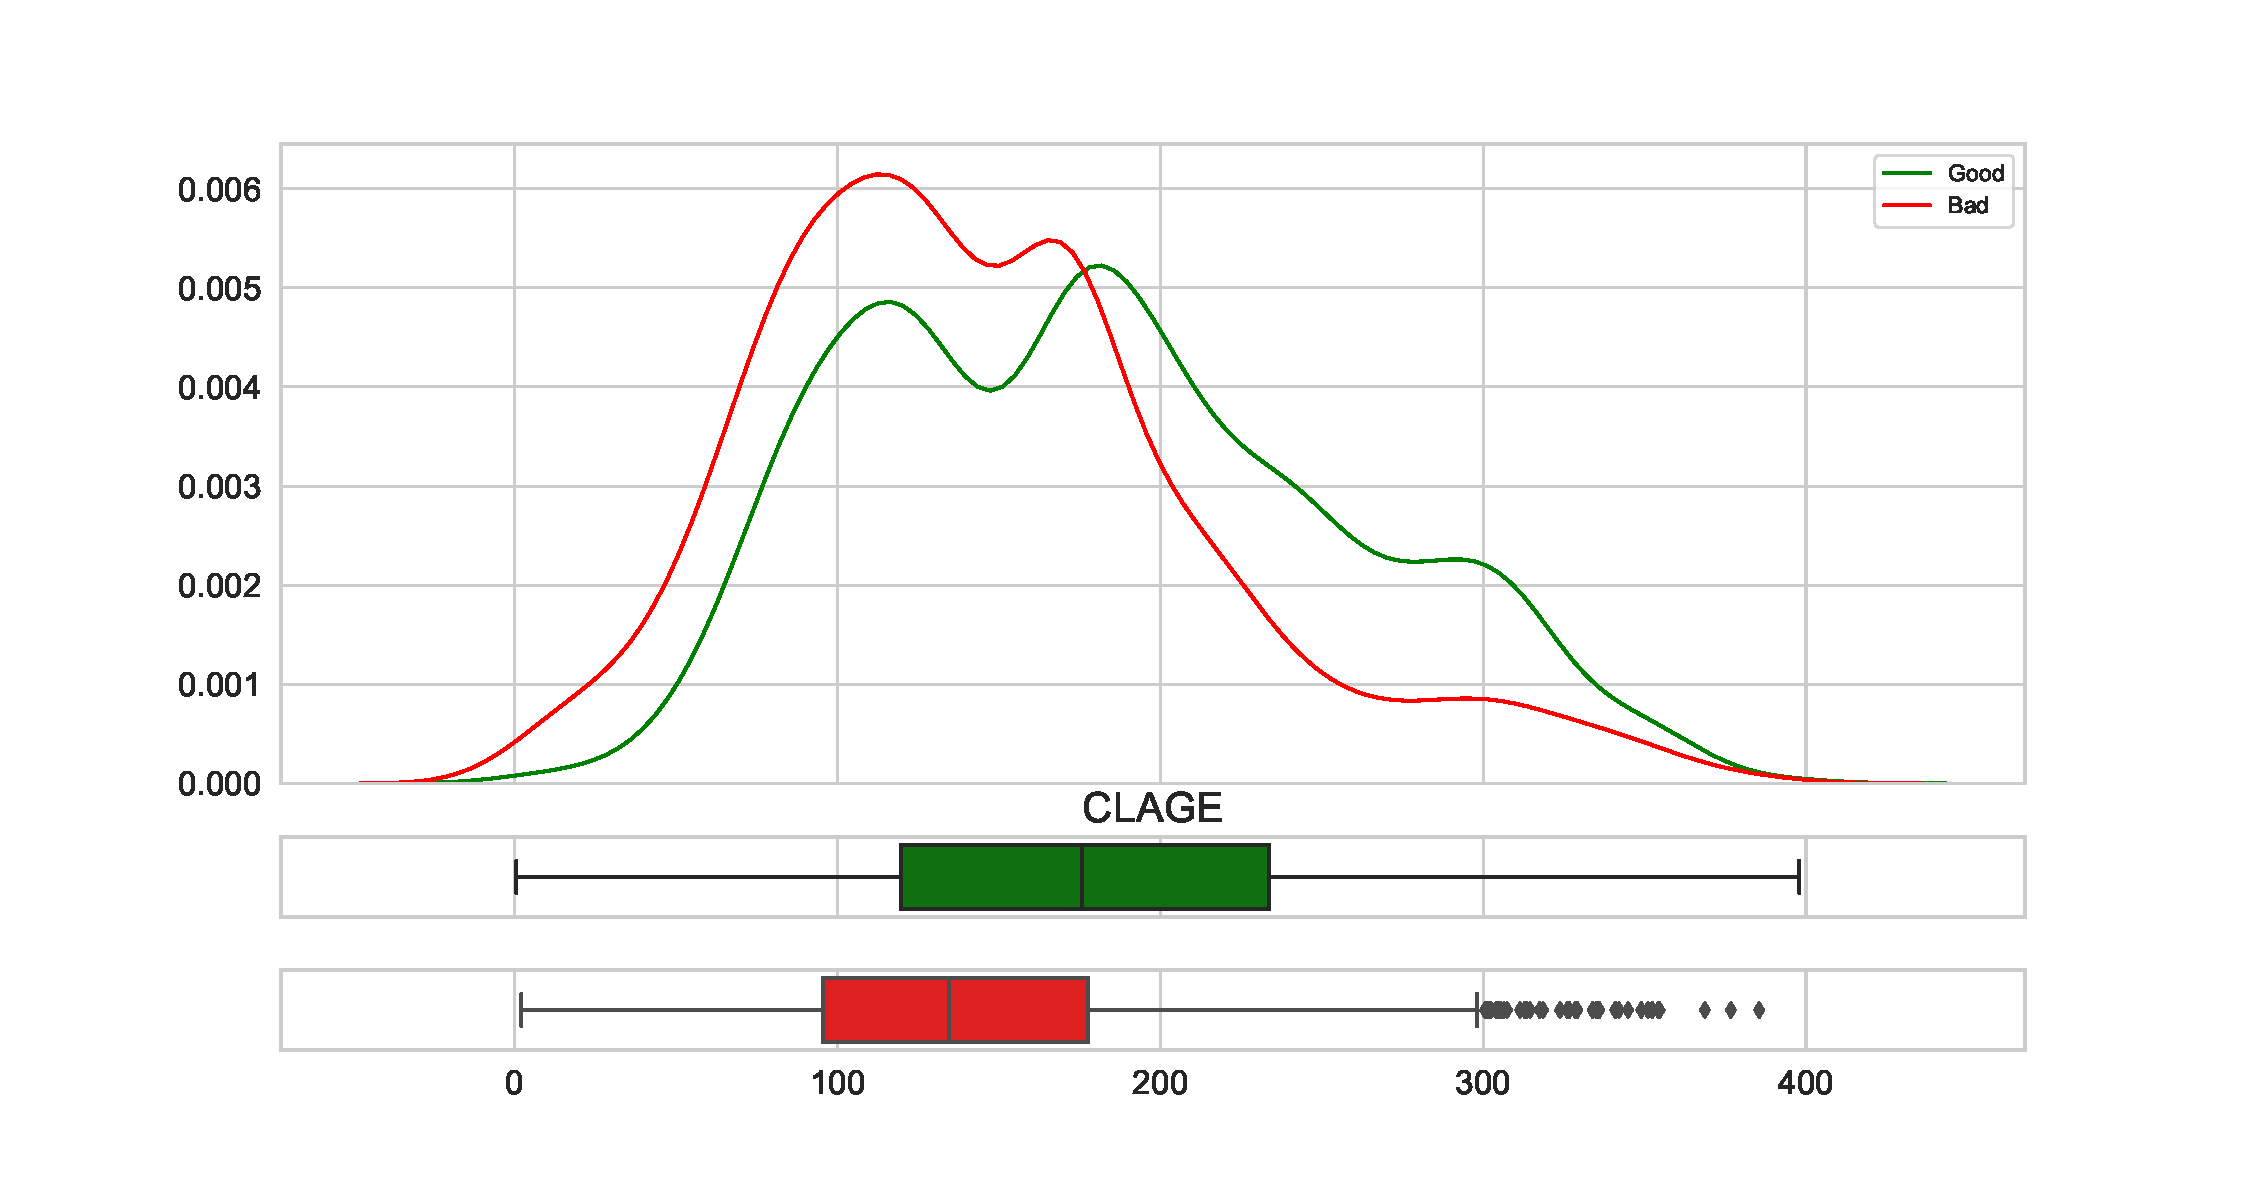
\includegraphics[scale=0.40]{figs/clage_dist.pdf}
	\caption{Distribution of CLAGE by BAD. \label{clage_dist}}
\end{figure}

\begin{figure}[!ht]
	\centering
	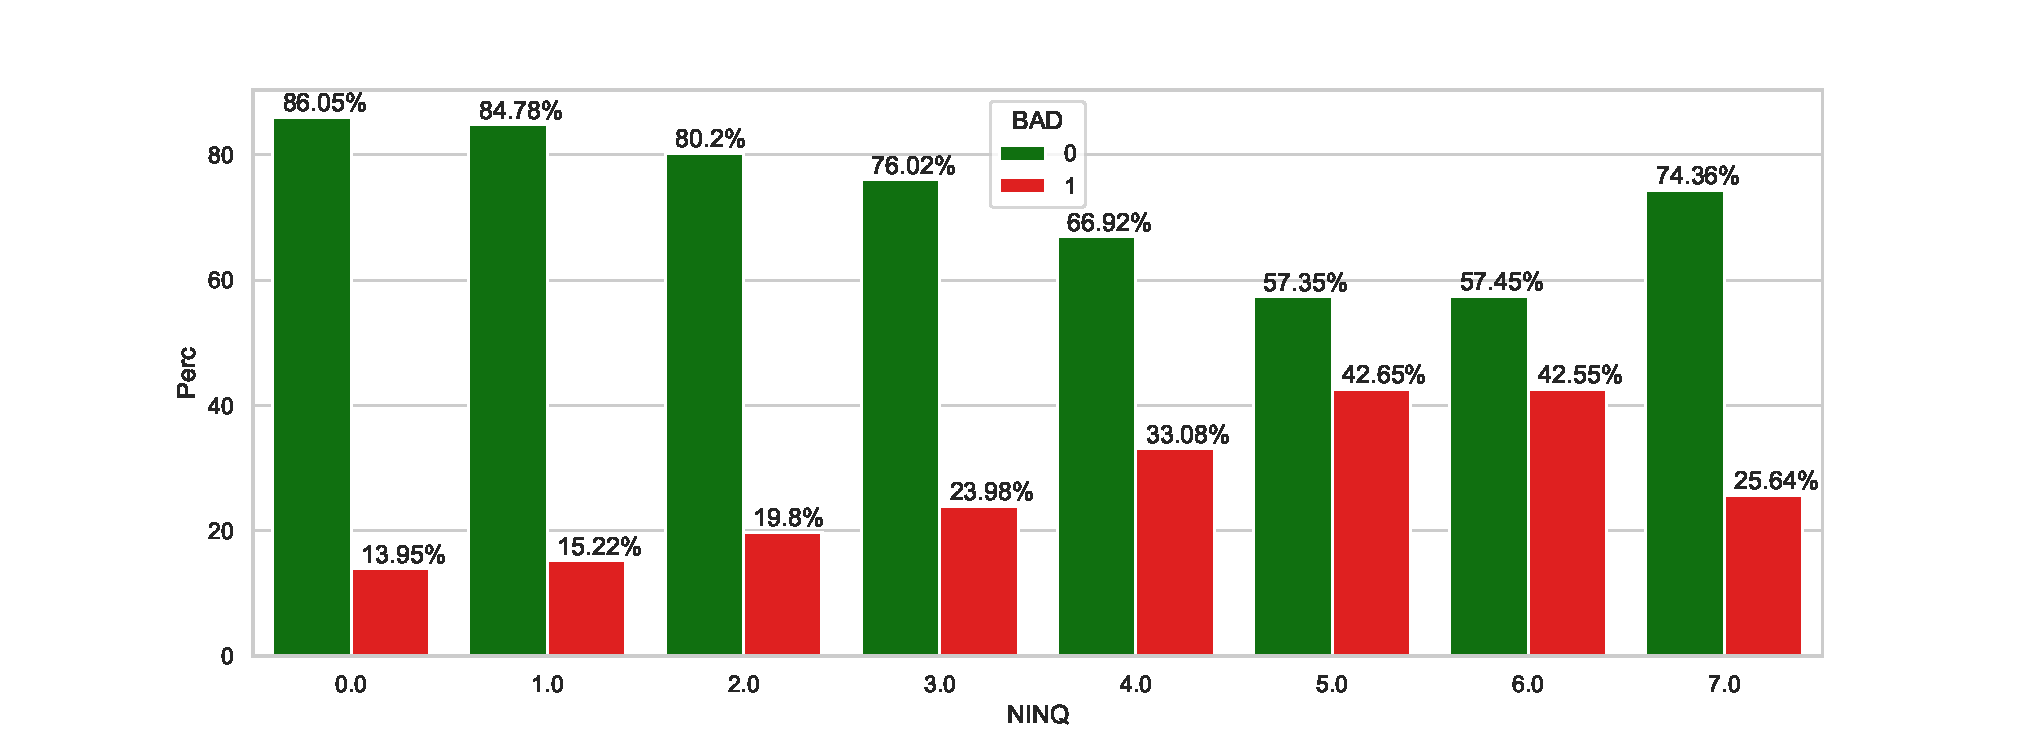
\includegraphics[scale=0.40]{figs/ninq_cat.pdf}
	\caption{Category plot of NINQ by BAD. \label{ninq_cat}}
\end{figure}

\begin{figure}[!ht]
	\centering
	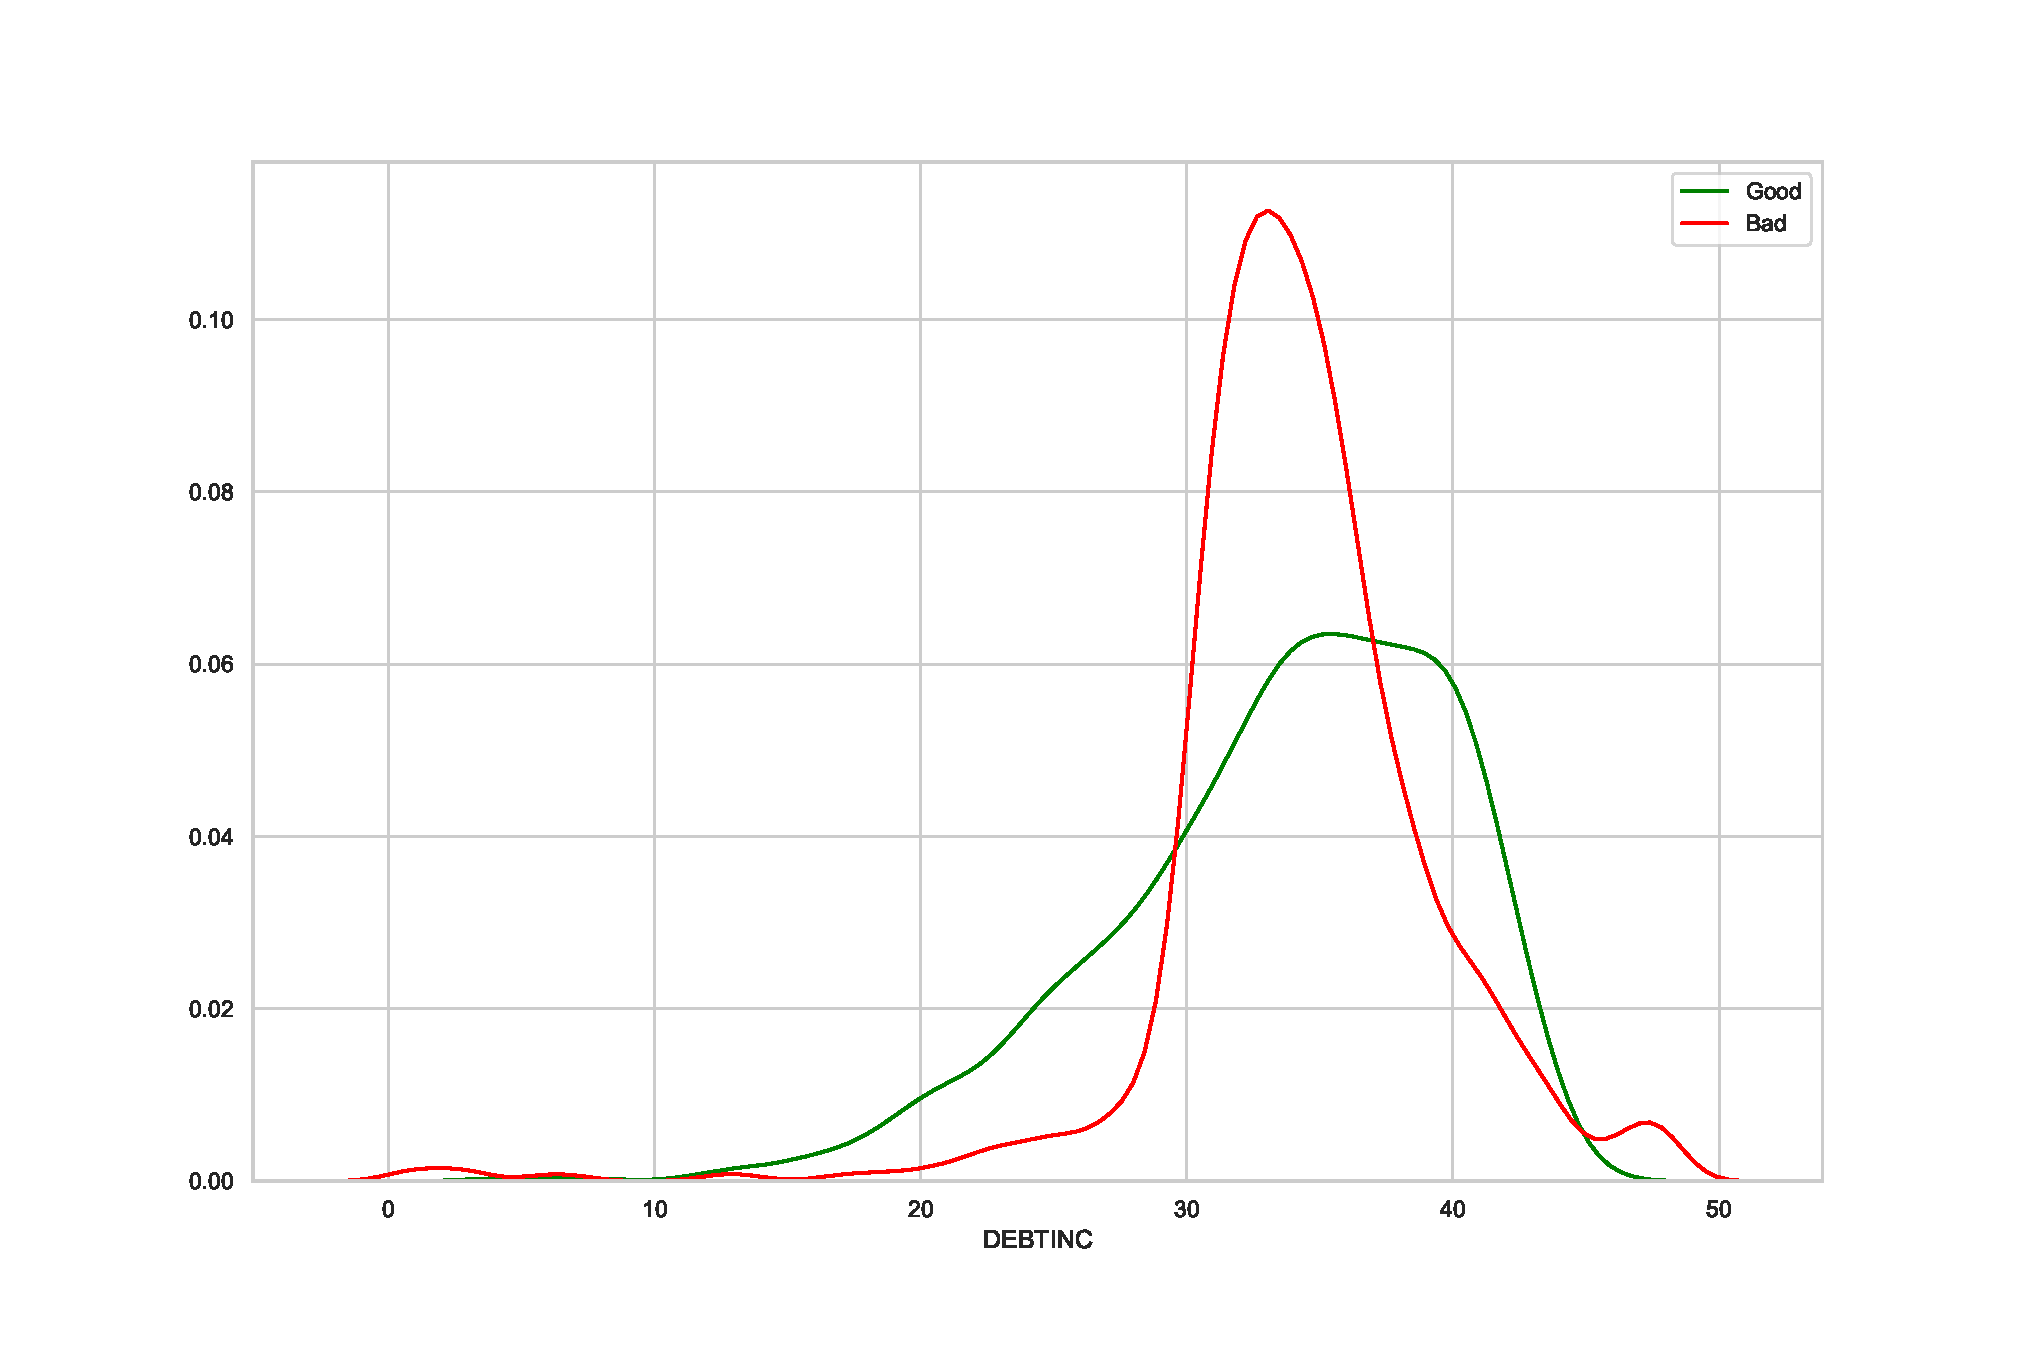
\includegraphics[scale=0.40]{figs/debtinc_dist.pdf}
	\caption{Distribution of DEBTINC by BAD. \label{debtinc_dist}}
\end{figure}


Breakdown of each variable go here.

\section{WOE and IV}

WOE results here.

IV results here.
%
%The data I am looking at was originally from the StatLib library maintained by Carnegie Mellon University. The data set was created and initially presented by Harrison, D. and Rubinfeld, D.L.\cite{harrison1978hedonic}\cite{gilley1996harrison}\cite{welsch1980regression} and since has been independently analyzed and used in multiple other papers. The data set was originally used to look into the willingness to pay for clean air and contains 506 observations of 14 variables. Median Value(MV) is the observed median value of a house in that area which will be our response variable.
%
%\begin{figure}[ht]\label{Table2}
%	\renewcommand{\arraystretch}{1.25}
%	\begin{tabular}{l p{6.8cm} p{5cm}}
%	\multicolumn{3}{c}{Variables used in the Data Set}\cite{harrison1978hedonic}\\
%	\hline
%	Variable & \multicolumn{1}{c}{Definition} & \multicolumn{1}{c}{Source}\\ \hline
%	CRIM & Crime rate by town & FBI (1970)\\
%	ZN & Proportion of residential land zoned for lots over 25,000 sq ft & Metropolitan Area Planning Com (1972)\\ 
%	INDUS & Proportion of nonretail business acres per town & Vogt, Ivers, and Associates\\
%	CHAS & Charles River dummy: =1 if tract bounds river =0 if otherwise & 1970 U.S. Census Tract maps\\
%	NOX & Nitrogen oxide concentrate & TASSIM\\
%	RM & Average number of rooms per dwelling & 1970 U.S. Census\\
%	AGE & Proportion of houses built before 1940 & 1970 U.S. Census\\
%	DIS & Weighted distances to five employment centres & \\
%	RAD & Index of accessibility to radial highways & MIT Boston Project\\
%	TAX & Full value property tax rate & Massachusetts Taxpayers Foundation (1970)\\
%	PTRATIO & Pupil-teacher ratio by town & Massachusetts Dept. of Education (1971-1972)\\
%	B & Black proportion of the population & 1970 U.S. Census\\
%	LSTAT & Proportion of the population that is lower status & 1970 U.S. Census\\
%	MV & Median Value & 1970 U.S. Census\\ 
%	\end{tabular}
%\end{figure}
%
%\begin{figure}[!ht]
%	\centering
%	\renewcommand{\arraystretch}{2.8}
%	\begin{tabular}{l r r r r r r r r r r r r r r}
%			&Min	&1st Qu.	&Median	&Mean	&3rd Qu.	&Max\\
%	CRIM    &0.006	&0.082		&0.257	&3.614	&3.677	&88.98\\
%	ZN      &0.000 	&0.000		&0.000	&11.36	&12.50	&100.0\\
%	INDUS   &0.460	&5.190		&9.690	&11.14	&18.10	&27.74\\
%	CHAS    &0.000	&0.000		&0.000	&0.069	&0.000	&1.000\\
%	NOX     &0.385	&0.449		&0.538	&0.555	&0.624	&0.871\\
%	RM      &3.561	&5.886		&6.208	&6.285	&6.623	&8.780\\
%	AGE     &2.900	&45.02		&77.50	&68.57	&94.08	&100.0\\
%	DIS     &1.130	&2.100		&3.207	&3.795	&5.188	&12.13\\
%	RAD     &1.000	&4.000		&5.000	&9.549	&24.00	&24.00\\
%	TAX     &187.0 	&279.0		&330.0	&408.2	&666.0	&711.0\\
%	PTRATIO &12.60	&17.40		&19.05	&18.46	&20.20	&22.00\\
%	B       &0.32	&375.4		&391.4	&356.7	&396.2	&396.9\\
%	LSTAS   &1.730	&6.950		&11.36	&12.65	&16.95	&37.97\\
%	MEDV    &5.000	&17.02		&21.20	&22.53	&25.00	&50.00\\
%	\end{tabular}
%	\caption{Summary Table \label{Table3.1}}
%\end{figure}
%
%\section{Variables}
%
%
%\subsection*{Per capita crime rate by town}
%The crime rate in Boston when viewed by City-Data's crime index in 2014 was reported to be just higher than the national average\cite{CityDataCrime} and has a violent crime rate of 396.4 per 100,000 people and a property crime rate of 216.5 per 100,000 people compared to the National averages of 200.7 and 230.8 respectively so even though violent crime is almost double the national average, property crime is lower than the average in Boston. \\
%
%Crime can be seen to have a substantial effect when considering the value of a house. Usually, when a buyer is searching for a property, having a high crime rate in the neighbourhood is a strong deterrent especially if that crime rate is particularly high in property based crimes. In a 2012 report by the Center for American Progress they found that just a $10\%$ reduction in the homicide rate in an area can increase the property value by $0.83\%$.\cite{maximino2014impact} So the initial assumption which I am going to make is that the crime rate will have a strong negative effect on the value of the housing.\\
%
%When looking at the crime rates given in our data set, the majority of the crime rates come between 0-1\% with a median value of $0.25651$ and is seen to decrease rapidly after going above 1\% with only 25\% of the data points recorded above 3.677\% crime rate. The correlation with the median value has a value of -0.3883046 which supports our initial assumption. I decided, when plotting CRIM against MEDV, to use the logarithmic form of CRIM for a better visualisation (\ref{CRIM}) as we can see there is a trend downwards in the median value of the houses as the crime rate increases in the town the housing was taken from. 
%
%\begin{figure}[!ht]
%	\centering
%	\includegraphics[scale=0.40]{figs/CRIM_Graphic.pdf}
%	\caption{Per capita crime rate by town. \label{CRIM}}
%\end{figure}
%
%\subsection*{Prop of residential land zoned for lots over 25,000 sq.  ft.}
%
%Having a larger proportion of residential land zoned for lots over 25,000 sq. ft. in a town suggests more of the housing will be contained in suburban style housing instead of terraced or apartment style housing. Housing of this type are usually to be valued more due to the house being more spacious and a reduction in noise due to being detached. This idea is supported when looking at the "Recent empirical work on the determinants of relative house prices" study\cite{ball1973recent} and studies numbered 3 and 4 by Apps and Cubbin, in their hedonic price models they both found that larger plots for housing had a positive coefficient for predicting the value of the housing. Specifically in Cubbin's having the houses split categorically for the type of housing (Flat, Semi-detached, Detached), Flat had a negative effect of $-\$391$ and Detached had a positive effect of $\$1014$.\\
%
%Considering our data it can be seen that most of the data is taken in areas of low proportions, infact the majority of areas have a proportion of $0$ and a median value of $0$ which is to be expected if most of the data is coming from the more central parts of Boston i.e. the city itself. we also get a small correlation of $0.3604453$. From this I am going to make the assumption that ZN will have a small positive affect on the value of the properties. 
%
%\begin{figure}[!ht]
%	\centering
%	\includegraphics[scale=0.40]{figs/ZN_Graphic.pdf}
%	\caption{Prop of residential land zoned for lots over 25,000 sq.  ft. \label{ZN}}
%\end{figure}
%
%\newpage
%
%\subsection*{Prop of non-retail business acres per town}
%
%Non-retail business acres could be causes of the production of various types of pollutions such as noise, air or visual pollutions from certain industries built on the acres. These could impact the values of housing around the areas due to the various unwanted pollutions.\\
%
%Taking the data which we have into consideration most of the areas the data has been gathered from contain around 5-15\% of non-retail acres. A lot of the data can be seen to be taken from areas with 18.10\% of non-retail acres. We can see that there is a negative trend for the value of our properties as the proportions of these acres increases and we have median proportion of $9.69$ and a correlation of $-0.4837252$ further backing our assumption that this variables coefficient will have a negative sign.
%
%\begin{figure}[ht]
%	\centering
%	\includegraphics[scale=0.40]{figs/INDUS_Graphic.pdf}
%	\caption{Prop of non-retail business acres per town \label{INDUS}}
%\end{figure}
%
%\subsection*{Charles River dummy variable}
%
%The Charles river dummy variable is an indication of whether or not the property is on the side of a river, with 0 as not being adjacent and 1 with the property being adjacent. A riverside property is usually valued more for owners and will most likely have higher property value.\\
%
% Looking at figure (\ref{CHAS}), There is a clear effect on property values when on the riverside although it is a rather small positive effect. The coefficient on this variable should be positive although due to small correlation $0.1752602$ I expect the variable selection methods to remove this early on.
%
%\begin{figure}[!ht]
%	\centering
%	\includegraphics[scale=0.40]{figs/CHAS_Graphic.pdf}
%	\caption{Charles River dummy variable \label{CHAS}}
%\end{figure}
%
%\subsection*{Nitric oxides concentration}
%
%Nitric oxide concentration was included in the original data because Harrison and Rubinfeld were looking into the demand for clean air. Another similar study on the demand for clean air for Seoul, Korea\cite{kim2003measuring} produced similar results as Harrison and Rubinfeld, in that an improvement in air quality results in higher median values for the properties.\\
%
%Nitric oxide concentration is an indication of the air quality in the area due to the collection of pollutant gases. These gases are an after product of fuel being burnt at high temperatures, often produced by vehicles and certain industries. There is a more indepth explanation of the effects of these gases in the area of New England on the EPA's website\cite{NOX}. This variable should see high values in areas with industrial complexes and high traffic areas such as highways which could be why we see high correlations between this value and INDUS and RAD with $0.764$ and $0.611$ respectively.\\
%
%In our data the concentrations range from $0.3850$ to $0.8710$ and as I can see, median value of the housing has a negative trend as the concentration increases. Although this may just be because concentrations are higher in more urban areas or industrial areas, I expect this variable to have a negative coefficient in the produced models.
%
%\begin{figure}[!ht]
%	\centering
%	\includegraphics[scale=0.40]{figs/NOX_Graphic.pdf}
%	\caption{Nitric oxides concentration \label{NOX}}
%\end{figure}
%
%\newpage
%
%\subsection*{Average number of rooms per dwelling}
%
%Average number of rooms indicates the amount of space and the size of the house and this can be expected to have a positive effect on the value of a property. In a collection of studies\cite{ball1973recent}, all of the papers include some type of value such as floor area, number of bedrooms, total rooms which can be considered similar to average number of rooms. In one of the American studies done by Ridker and Henning\cite{ridker1967determinants}, their variable was median number of rooms, where the addition of one room produced an increase in value of $\$284.10$ for the property.\\
%
%When looking at our data in figure (\ref{RM}). we can see similar trends to that of the other studies. The median number of rooms is 6.2085 and most of the houses in our data have either 6 or 7 rooms. Plotted against the median value of our houses there is a strong indication that the value of the property is dependent on the number of rooms in the property so I can expect this variable will have a positive coefficient.
%
%\begin{figure}[!ht]
%	\centering
%	\includegraphics[scale=0.40]{figs/RM_Graphic.pdf}
%	\caption{Average number of rooms per dwelling \label{RM}}
%\end{figure}
%
%\subsection*{Prop of owner-occupied units built prior to 1940}
%
%The age of a property is an important consideration when looking into a property, the style of the house can be linked to the date of construction which can often be valued in a house. The age of the house can also to be linked to quality of the structure, the older a house is can lead to a deterioration in structural integrity and require maintanence. Looking at the other recent studies on property values,\cite{ball1973recent} whenever the age of the structure is included in these studies, it produces a negative coefficient. Specifically in Kain and Quigley's study\cite{kain1970measuring}, a year increase in the age of a property has the effect of reducing the property's value by $0.088\%$\\
%
%Our data does not provide us with the specific ages of properties in the area, only the proportion of them that have been built before 1940 although I believe the other studies data on age still gives us a good idea of what this variable's coefficient will be. Considering this when looking at the data I have, the higher the proportion of units which have been built prior to 1940 seems to have a negative effect on the median values of our properties, you can see this when looking at figure (\ref{AGE}). This is probably an indication that the older properties in the areas taken are valued less and are therefore dragging the median value down. I am expecting AGE to have a negative coefficient.
%
%\begin{figure}[!ht]
%	\centering
%	\includegraphics[scale=0.40]{figs/AGE_Graphic.pdf}
%	\caption{Prop of owner-occupied units built prior to 1940 \label{AGE}}
%\end{figure}
%
%\subsection*{Weighted distances to five Boston employment centers}
%
%Employment centers are more likely to have a higher density as you reach closer to the city and it's center. So housing closer to the center of the city will most likely have lower weighted distances to five employment centers. This is supported when we compare the census tracts with the observations. The Boston census tract are the observations 357 - 488 have a DIS mean of $2.061254$ compared to the overall mean of $3.795043$.\\
%
%The more central a housing is the more likely it will be more urban style housing such as apartments which are generally of lower value. Looking at our data, most of our observations are between 1 and 5 weighted distance from five employment centers and looking at figure(\ref{DIS}), we can see a strong linear trend in distances 1 to 2.5 and then our data points become more spread most likely indicating the observations outside of the urban areas.
%
%\begin{figure}[!ht]
%	\centering
%	\includegraphics[scale=0.40]{figs/DIS_Graphic.pdf}
%	\caption{Weighted distances to five Boston employment centers \label{DIS}}
%\end{figure}
%
%\newpage
%
%\subsection*{Index of accessibility to radial highways}
%
%A high index is seen to be an indication of a higher urban area and less suburban. A higher urban area is going to have limited zones for property, smaller properties are more likely to have lower property values.\cite{ball1973recent} Along with higher urban area, a high index is likely to mean a closer proximity to highways. A recent study done by Jon P. Nelson on the effect of highway noise and property values show that being close to the cause of noise pollutions is more likely going to reduce the values of properties.\cite{nelson1982highway}
%
%\begin{figure}[!ht]
%	\centering
%	\includegraphics[scale=0.40]{figs/RAD_Graphic.pdf}
%	\caption{Index of accessibility to radial highways \label{RAD}}
%\end{figure}
%
%\subsection*{Full-value property-tax rate per \$ 10,000}
%
%In the study by Wallace E. Oates on "The Effects of Property Taxes and Local Public Spending on Property Values", he discovered that property tax has a significant negative effect on the housing values when unaccompanied by an increase in the output of local public services.\cite{oates1969effects} Our data suggests the same with a correlation of $-0.469$ we can expect this coefficient to be negative in the models
%
%\begin{figure}[!ht]
%	\centering
%	\includegraphics[scale=0.40]{figs/TAX_Graphic.pdf}
%	\caption{Full-value property-tax rate per \$ 10,000 \label{TAX}}
%\end{figure}
%
%\subsection*{Pupil-teacher ratio by town}
%
%School quality has been seen as a great factor in when purchasing a property. In a study done by G. Donald Jud and James M. Watts\cite{jud1981schools} they came to the conclusion that an increase of one grade level in achievement level can increase the average value of a house from 5.2\% to 6.2\%. A low Pupil-teacher ratio creates more one on one time with students with fewer students a teacher has to handle. More one on one time is known to increase the students quality of learning. Looking at the data I have in figure (\ref{PTRATIO}). I am expecting this variable to have a positive coefficient in my models.
%
%\begin{figure}[!ht]
%	\centering
%	\includegraphics[scale=0.40]{figs/PTRATIO_Graphic.pdf}
%	\caption{Pupil-teacher ratio by town \label{PTRATIO}}
%\end{figure}
%
%\subsection*{Prop of blacks by town}
%
%Many studies such as the one done by David R. Harris\cite{harris1999property} find that neighbourhoods with high percentages of blacks have a reduction in housing values. The reason for this is still debated, reasons could be that other races report their unwillingness to have black neighbours or that people prefer living within neighbourhoods of well-educated people which are more common in other races.\\
%
%In the original study, they decide that the black proportion is going to have a parabolic effect on the property value as an increase in black population in an area with a small population already is going to have a negative effect on property value and due to discrimination, areas with high black population is going to have a higher property value. To produce this effect they created the data we have now which is $B = (Bk - 0.63)^2$ where Bk is the proportion of blacks in the area. Looking at the data on figure (\ref{B}), due to almost all our data being in neighbourhoods of similar black proportions it's hard to make a determination from this if their assumption could be true. With the proportions of black people being fairly low, I expect this to produce a negative coefficient.
%
%\begin{figure}[!ht]
%	\centering
%	\includegraphics[scale=0.40]{figs/B_Graphic.pdf}
%	\caption{$(Bk - 0.63)^2$ where Bk is the proportion of blacks by town \label{B}}
%\end{figure}
%
%\subsection*{\% lower status of the population}
%
%In the original paper containing this data lower status was assigned to the proportion of adults without some high school education and proportion of male workers classified as laborers. Due to the limited type of employment an adult can get without high school level qualifications means they will have a limited amount of income. This will most likely mean the value of their property is going to be also at a lower value. Therefore a higher proportion of lower status population in an area is going to bring down the median value of the housing in that area.\\
%
%Looking at the data we have and figure (\ref{LSTAS}), the areas in the data contain an average of \%12 at lower status and a median of 11.36. When we compare this to our median value in those areas we can see a strong decline in the value of the houses as the proportion of lower status population increases. I expect this variable to be significant in our model and to have a negative coefficient. 
%
%\begin{figure}[!ht]
%	\centering
%	\includegraphics[scale=0.40]{figs/LSTAS_Graphic.pdf}
%	\caption{lower status of the population \label{LSTAS}}
%\end{figure}
%
%\subsection*{Median value of owner-occupied homes in \$ 1000's}
%
%Median value is our response variable and the variable I would like to predict. The mean value of our observations is $\$22,532$ and the smallest median value we have is $\$5,000$. The maxmimum of median values appears to be censored at $\$50,000$ as there is 16 data points at exactly $\$50,000$. 
%
%
%\begin{landscape}
%\begin{figure}[ht]
%	\centering
%	\renewcommand{\arraystretch}{2}
%	\begin{tabular}{l r r r r r r r r r r r r r r}
%			&CRIM	&ZN		&INDUS	&CHAS	&NOX	&RM		&AGE	&DIS	&RAD	&TAX	&PTR	&B		&LSTAS	&MEDV\\
%	CRIM    &1.000	&		&		&		&		&		&		&		&		&		&		&		&		&\\
%	ZN      &-0.200	&1.000	&		&		&		&		&		&		&		&		&		&		&		&\\
%	INDUS   &0.406	&-0.534	&1.000	&		&		&		&		&		&		&		&		&		&		&\\
%	CHAS    &-0.056	&-0.043	&0.063	&1.000	&		&		&		&		&		&		&		&		&		&\\
%	NOX     &0.421	&-0.517	&0.764	&0.091	&1.000	&		&		&		&		&		&		&		&		&\\
%	RM      &-0.219	&0.312	&-0.392	&0.091	&-0.302	&1.000	&		&		&		&		&		&		&		&\\
%	AGE     &0.353	&-0.570	&0.645	&0.087	&0.731	&-0.240	&1.000	&		&		&		&		&		&		&\\
%	DIS     &-0.380	&0.664	&-0.708	&-0.099	&-0.769	&0.205	&-0.748	&1.000	&		&		&		&		&		&\\
%	RAD     &0.626	&-0.312	&0.595	&-0.007	&0.611	&-0.210	&0.456	&-0.495	&1.000	&		&		&		&		&\\
%	TAX     &0.583	&-0.315	&0.721	&-0.036	&0.668	&-0.292	&0.506	&-0.534	&0.910	&1.000	&		&		&		&\\
%	PTRATIO &0.290	&-0.392	&0.383	&-0.122	&0.189	&-0.356	&0.262	&-0.232	&0.465	&0.461	&1.000	&		&		&\\
%	B       &-0.385	&0.176	&-0.357	&0.049	&-0.380	&0.128	&-0.274	&0.292	&-0.444	&-0.442	&-0.177	&1.000	&		&\\
%	LSTAS   &0.456	&-0.413	&0.604	&-0.054	&0.590	&-0.614	&0.602	&-0.497	&0.489	&0.544	&0.374	&-0.366	&1.000	&\\
%	MEDV    &-0.388	&0.360	&-0.484	&0.175	&-0.427	&0.695	&-0.377	&0.250	&-0.382	&-0.469	&-0.508	&0.333	&-0.738	&1.000\\
%	\end{tabular}
%	\caption{Correlation Table \label{Table3}}
%\end{figure}
%\end{landscape}
%
%\section{Correlation and Multicollinearity}
%
%\paragraph{\textbf{Full property value tax and Index of accessibility to radial highways}}
%
%TAX and RAD are the highest correlated variables in the data set but when looking at the data it appears the correlation is skewed due to the problem that 131 observations have been taken in the same area. giving more than 131 observations with the value of 24 and 666 for RAD and TAX respectively. This could be quite a problem, if they have all been taken from the same town then these 131 data points are heavily skewing our data. We can see where this data has come from by looking at in the paper "Regression Sensitivity Analysis and Bounded-Influence Estimation" where table 2 provides the census tracts. Our data with identical RAD and TAX are observations 357-488 and which have all been taken from Boston city and then separated by individual parts of Boston. For those observations some of the data have been taken at town level and some have been taken city wide such as ZN, INDUS, RAD, TAX and PTRATIO. \\
%
%This is could be quite a probem as it is causing incorrect correlations between our variables.\cite{welsch1980regression} when you look at the correlations of TAX and RAD when those data points are removed it goes from $0.910$ to $0.250$. You can see the effect this is having on the relationship between the two when using the R function coplot.  Since it is not specified how the data points were collected, there is no indication that these are all individual recorded points or if they took the point from the entire of boston and used it for all the individual towns. In figures (\ref{TAXRAD1}) and (\ref{TAXRAD2}) you can see when taking all the data points the relationship is heavily affected by the points from the city. When removing those points the change in density of the MEDV points is fairly unchanged but the relationship between RAD and TAX becomes far less significant and the subset show more visible change in the relationship.\\
%
%One option is to remove those observations but that would be a large loss of information from an already small sample of data and removing the data coming from the Boston census tract removes a quarter of our data. Another option can be to remove some of the affected variables from the data but there are problems which come with this as well, such as increased bias in the other estimates. Another option would be to just leave the data as it is and allow the methods to deal with this for us. 
%
%\paragraph{\textbf{Multicollinearity}}
%
%As you can see from figure (\ref{Table3}) a lot of our predictors have high correlations between each other. This can be a large problem if not checked. To look into this I decided to use the variable inflation factor(vif) function in the package DAAG\cite{maindonald2015package} to test if multicollinearity could be a problem in my models. The variable inflation factor is an indicator of how much the variance of an estimated coefficient increases due to collinearity.
%
%\begin{lstlisting}[language=R]
%library(DAAG)
%vif.test <- lm(y ~ x)
%vif(test)
%\end{lstlisting}
%
%The results of this function can be seen in figure (\ref{Table4}). With all data included some of the inflation factors returned very high, for instance TAX and RAD. This factor is an indication of how many times larger the varaince is for that particular coefficient. So with TAX $9.0086$ means that the variance on the TAX coefficient is 9 times larger than what it would be if it was completely uncorrelated with all other variables. Ideally I want these factors as small as possible and there is a few ways in which you can reduce variable inflation, one of those ways is by removing one of the highly correlated predictors which may likely be causing the problem.\\
%
%I decided to remove the variable TAX to see how the factors change. The results of that are in the second column. RAD's factor ended up being reduced by $4.6$ which was to be expected since TAX and RAD had a skewed correlation of $0.910$, as talked about earlier, this correlation may not be entirely accurate. This brought all our variables below a factor of 5. I also decided to run a model removing the next variable with the highest factor which was NOX. This can be seen in the third column. Removing this did not have a large effect on the other variables but this did bring all of our factors to below 4 which means all of our variables standard errors are increased by no more than 2 times due to multicollinearity. There is a problem with dropping variables to reduce multicollinearity. Dropping the variable will result in loss of information when fitting the model and most likely reducing the accuracy of the model but it can help with producing more significant variables which is what we are interested in. Robert M. O’Brien talks about being cautious about removing variables\cite{o2007caution} to reduce this factor as in turn it can produce more problems and recommends not removing a variable without taking these problems into consideration.
%
%\begin{figure}[ht]
%	\centering
%	\begin{tabular}{l r r r}
%			&Set 1		&Set 2 		&Set 3\\
%	CRIM	&1.7922		&1.7919		&1.7853\\
%	ZN		&2.2988		&2.1842		&2.1834\\
%	INDUS	&3.9916		&3.2260		&2.8728\\
%	NOX		&4.3937		&4.3693		&.\\
%	RM		&1.9337		&1.9231		&1.9040\\
%	AGE		&3.1008		&3.0980		&2.8751\\
%	DIS		&3.9559		&3.9544		&3.6415\\
%	RAD		&7.4845		&2.8375		&2.5336\\
%	TAX		&9.0086		&.			&.\\
%	PTRATIO	&1.7991		&1.7888		&1.5989\\
%	B		&1.3485		&1.3476		&1.3396\\
%	LSTAS	&2.9415		&2.9408		&2.9273\\
%	CHAS	&1.0740		&1.0582		&1.0576\\
%	\end{tabular}
%	\caption{Variable Inflation Factor Table \label{Table4}}
%\end{figure}
%
%\begin{figure}[ht]
%	\centering
%	\includegraphics[scale=0.40]{figs/TAXRAD2.pdf}
%	\caption{Coplots of original Data \label{TAXRAD1}}
%\end{figure}
%
%\begin{figure}[ht]
%	\centering
%	\includegraphics[scale=0.40]{figs/TAXRAD3.pdf}
%	\caption{Coplots when boston city is removed \label{TAXRAD2}}
%\end{figure}
%
